
%% RSET Project / Seminar LaTex Template Version 1.0 - November 2023

\documentclass[12pt,a4paper,titlepage]{report}
\usepackage{graphicx}
\usepackage[left=2.8cm, right=2.2cm, top=3cm, bottom=2.5cm]{geometry}
\usepackage{latexsym}		% to get LASY symbols
\usepackage{epsfig}			% to insert PostScript figures
\usepackage{eufrak}
\usepackage{type1cm}
\usepackage{newsec}
\usepackage{titlesec}
\usepackage{longtable}
\usepackage{url}
\usepackage[export]{adjustbox}
\usepackage{listings}
\usepackage{xcolor}
\usepackage{pdfpages}
\usepackage{caption}
\usepackage{listings}
\usepackage{float}
\usepackage{acro}
\usepackage{setspace}
\usepackage{caption}
\usepackage{subcaption}

\definecolor{customgreen}{rgb}{0,0.6,0}
\definecolor{customgray}{rgb}{0.5,0.5,0.5}
\definecolor{custommauve}{rgb}{0.6,0,0.8}
\lstdefinelanguage{HTML}{
	sensitive=true,
	keywords={},
	otherkeywords={<, >, /},
	morecomment=[s]{<!--}{-->},
	morestring=[b]"
}


\lstset{ 
	basicstyle=\small,        % the size of the fonts that are used for the code
	breaklines=true,                 % sets automatic line breaking
	commentstyle=\color{customgreen},    % comment style
	firstnumber=1,                % start line enumeration with line 1000
	frame=single,	                   % adds a frame around the code
	keepspaces=true,                 % keeps spaces in text, useful for keeping indentation of code (possibly needs columns=flexible)
	keywordstyle=\color{blue},       % keyword style
	numbers=left,                    % where to put the line-numbers; possible values are (none, left, right)
	numbersep=10pt,                   % how far the line-numbers are from the code
	numberstyle=\tiny\color{customgray}, % the style that is used for the line-numbers
	rulecolor=\color{black},         % if not set, the frame-color may be changed on line-breaks within not-black text (e.g. comments (green here))
	showspaces=false,                % show spaces everywhere adding particular underscores; it overrides 'showstringspaces'
	showstringspaces=false,          % underline spaces within strings only
	showtabs=false,                  % show tabs within strings adding particular underscores
	stepnumber=1,                    % the step between two line-numbers. If it's 1, each line will be numbered
	stringstyle=\color{custommauve},     % string literal style
	tabsize=2,	                   % sets default tabsize to 2 spaces
	title=\lstname                   % show the filename of files included with \lstinputlisting; also try caption instead of title
}


\titleformat{\chapter}[display]
{\normalfont\Large\bfseries\centering}{\chaptertitlename\
	\thechapter}{25pt}{\Large}
\titleformat{\section}{\normalfont\bfseries}{\noindent\thesection}{20pt}{}
\titleformat{\subsection}{\normalfont\small\bfseries}{\thesubsection}{15pt}{\small}
\titlespacing*{\chapter}{0pt}{0pt}{40pt}
\usepackage{hyperref}
\usepackage{url}


\begin{document}
    
	\titlepage
	\thispagestyle{empty}
% \input{Chapters/vishwanath_titlepage.tex}
% \input{Chapters/serah_titlepage.tex}
% 	\begin{center}
		
\includegraphics[scale=0.1]{Images/logo1.png}\\[0.5cm]
		\large \textit{Project Report on}\\[0.5cm]
		\Large \textbf{Multiplayer Narrative Driven Game using Memory Augmented LLM for Real-Time Social Deception}\\[0.4cm]
		\textit{Submitted in partial fulfillment of the
			requirements for the award of the degree of}\\[0.5cm]
		{\huge {$\mathfrak {Bachelor\; of\; Technology}$}}\\[.6cm]
		%{\Large {$\mathfrak {In}$}}\\[.5cm]
		%{\Large {$\mathfrak {Computer\; Science\; \&\; Engineering}$}}\\[2cm]
		\textit{in}\\[0.4cm]
		{\Large \bf \itshape{{Computer Science and Engineering}}}\\[0.4cm]
		\large \bfseries{By}\\[.6cm]
		% \large \bfseries{ Vishwanath Pradeep (U2203212) }\\[0.6cm]
		% \large \bfseries{ Serah Grace Kurian (U2203192) }\\[0.2cm]
		\large \bfseries{ Nandhaakishore S (U2203149) }\\[0.2cm]
		% \large \bfseries{ Sreenandan Pradeep (U2203199) }\\[0.4cm]
		\large \bfseries{Under the guidance of}\\[0.6cm]
		\large \bfseries{Mr. Sebin Jose\\Assistant Professor\\Dept. of CSE}\\[0.6cm]
%		\includegraphics[width=8.0cm]{logo (1).jpg}\\[0.5cm]
		\large \textbf{Department of Computer Science and Engineering}\\
		\large \textbf{Rajagiri School of Engineering \&\ Technology (Autonomous)}\\
		\small \bfseries{(Parent University: APJ Abdul Kalam Technological University)}\\
		\large \textbf{Rajagiri Valley, Kakkanad, Kochi, 682039}\\
		\large \bfseries{March 2026}
	\end{center}
	
	\newpage
	\thispagestyle{empty}
	\vspace{1cm}
	\begin{center}
	%	\textbf {DEPARTMENT OF COMPUTER SCIENCE \&\ ENGINEERING}\\
	%	\small \textbf{RAJAGIRI SCHOOL OF ENGINEERING \&\ TECHNOLOGY (AUTONOMOUS)}\\
	
	%	\small \textbf{RAJAGIRI VALLEY, KAKKANAD, KOCHI, 682039}\\
     %   \small \bfseries{(Affiliated to APJ Abdul Kalam Technological University)}\\[0.5cm]
		%\begin{figure}[htbp]
		%	\centering
			%\includegraphics[scale=0.40]{logo (1).jpg}
         %   \includegraphics[width=8.0cm]{logo (1).jpg}\\[0.5cm]
		%\end{figure}
		\large \bfseries{\huge{CERTIFICATE}}\\[1cm]
	\end{center}
	
	\renewcommand{\baselinestretch}{1.2}\normalsize
	
	\emph{This is to certify that the Project Report entitled \textbf{”Multiplayer Narrative Driven Game using Memory
Augmented LLM for Real-Time Social Deception”} is a bonafide record of the work done by 
% \textbf{Vishwanath Pradeep (U2203212)}, 
% \textbf{Serah Grace Kurian(U2203192)},
\textbf{Nandhaakishore S (U2203149)},
% and 
% \textbf{Sreenandan Pradeep (U2203199)},
submitted to the Rajagiri School of Engineering \& Technology (RSET) (Autonomous) in partial fulfillment of the requirements for the award of the degree of Bachelor of Technology (B. Tech.) in "Computer Science and Engineering" during the academic year 2025-2026.}\\[2.5cm]
	
\begin{flushleft}
	
	
	\begin{longtable}{p{10.8cm} p{10.8cm}}
	%	\small\textbf{Name of Guide}    &\small\textbf{Name of Coordinator} \\
        {\textbf{Project Guide}} &  {\textbf{Project Coordinator}}\\
		{Mr. Sebin Jose} & {Ms. Jisha Mary Jose}\\
		{Assistant Professor} & {Assistant Professor}\\
		{Dept. of CSE} & {Dept. of CSE}\\
		{RSET} & {RSET} \\
		
	\end{longtable}
\end{flushleft}
	
	\vspace{2cm}

\begin{flushleft}
	
	
	\begin{longtable}{p{5.8cm} p{5.8cm} p{5.8cm}}
	%	\small\textbf{Name of Guide}    &\small\textbf{Name of Coordinator} \\
		{}& {\textbf{Head of Department}} & {}\\
		{}& {Dr. Preetha K G} & {}\\
		{}& {Professor} & {}\\
		{}&  {Dept. of CSE} & {}\\
		{} ~&{RSET} & {} \\
		
	\end{longtable}
\end{flushleft}


%\begin{center}
%Name of HoD \\
%Designation \\
%Department Name \\
%RSET
%\end{center}
%\begin{flushleft}
%	
%	
%	\begin{longtable}{p{10.3cm} p{8cm} p{5.25cm}}
%	%	\small\textbf{Name of Guide}    &\small\textbf{Name of Coordinator} \\
%		{Project Coordinator}& {Name of HoD}\\
%		{Designation}& {Designation}\\
%		{Dept. Name}&  {Dept. Name}\\
%		{RSET} ~&{RSET} \\
%		
%	\end{longtable}
%\end{flushleft}

% \input{Chapters/sreenandan_titlepage.tex}
\input{Chapters/team_titlepage.tex}
	
	

    
	
\renewcommand{\baselinestretch}{1.5}\normalsize
\newpage
	%\renewcommand\abstractname{ACKNOWLEDGEMENTS}
% \input{Chapters/vishwanath_acknowledgements.tex}
% \input{Chapters/serah_acknowledgements.tex}
% \chapter*{ACKNOWLEDGMENT}
	\pagenumbering{roman}
	\setcounter{page}{1}
	\addcontentsline{toc}{chapter}{Acknowledgment}
	\vspace{1.5cm}
	\begin{spacing}{1}
		\paragraph\ I wish to express my sincere gratitude towards \textbf{Rev. Dr. Jaison Paul Mulerikkal CMI}, Principal of RSET, and \textbf{Dr. Preetha K G}, Head of the Dept. of CSE for providing me with the opportunity to undertake my project, Multiplayer Narrative Driven Game for Real-Time Social Deception.
		\paragraph\ I am highly indebted to my project coordinator, \textbf{Ms. Jisha Mary Jose}, Assistant Professor, Dept. of CSE, for her valuable support.
		
		\paragraph\ It is indeed my pleasure and a moment of satisfaction for me to express my sincere
		gratitude to my project guide \textbf{Mr. Sebin Jose} for his patience and all the priceless advice and  wisdom he has shared with me. 
		\paragraph\ Last but not the least, I would like to express my sincere gratitude towards all other teachers and friends for their continuous support and constructive ideas.

		% \paragraph\ We wish to express our sincere gratitude towards \textbf{Rev. Dr. Jaison Paul Mulerikkal CMI}, Principal of RSET, and \textbf{Dr. Preetha K G}, Head of the Dept. of CSE for providing us with the opportunity to undertake our project, Multiplayer Narrative Driven Game for Real-Time Social Deception.
		% \paragraph\ We are highly indebted to oure project coordinator, \textbf{Ms. Jisha Mary Jose}, Assistant Professor, Dept. of CSE, for her valuable support.
		
		% \paragraph\ It is indeed our pleasure and a moment of satisfaction for us to express our sincere gratitude to our project guide \textbf{Mr. Sebin Jose} for his patience and all the priceless advice and  wisdom he has shared with us. 
		% \paragraph\ Last but not the least, we would like to express our sincere gratitude towards all other teachers and friends for their continuous support and constructive ideas.
		
	\end{spacing}
	\begin{flushright}
		%\textbf{Vishwanath Pradeep}\\
		%\textbf{Serah Grace Kurian}\\
		\textbf{Nandhaakishore S}\\
		%\textbf{Sreenandan Pradeep}\\
	\end{flushright}
% \input{Chapters/sreenandan_acknowledgements.tex}
\input{Chapters/team_acknowledgements.tex}
		
		
\newpage
 
\renewcommand{\baselinestretch}{1.5}\normalsize
	
\chapter*{Abstract}
	%\begin{abstract}
	%	\pagenumbering{roman}
	%	\setcounter{page}{3}
		\addcontentsline{toc}{chapter}{Abstract}
		\vspace{1.5cm}

This project presents a 3D first-person multiplayer social deduction game set in a fictionalized Chernobyl Exclusion Zone, where players investigate mysterious disappearances as part of a government task force. Among them hides an alien organism capable of mimicry and deception, powered by a locally hosted, memory-augmented Large Language Model (LLM) that generates real-time, proximity-based chat to imitate players’ language patterns and emotional tones. Using a vector-based memory system (ChromaDB), the LLM maintains contextual awareness and behavioural consistency, adapting dialogue to sustain its disguise. Developed in Unity with multiplayer networking via Unity Netcode, the game features synchronized interactions and a Python backend handling LLM inference and memory retrieval. Local hosting ensures low latency and data privacy, enabling naturalistic deception, suspicion, and alliance-building among players. By integrating AI-driven dialogue, emotional modulation, and social reasoning, the project advances research in LLM-based autonomous agents, memory-augmented interaction, and computational models of trust and deception, with broader applications in simulation, storytelling, and AI-human interaction studies.    
		
		%\end{spacing}
	%\end{abstract}
	
	
	\newpage
	\normalsize{}
	
	%\pagenumbering{roman}
	%\setcounter{page}{4}
	%\begin{spacing}{}
	\tableofcontents
	%\end{spacing}
	% \thispagestyle{empty}
	\newpage
	
\chapter*{List of Abbreviations}
\addcontentsline{toc}{chapter}{List of Abbreviations}

\vspace{1cm}

\begin{tabbing}
% Adjusted tab spacing for tighter layout
HIN \hspace{5cm} \= \kill

\textbf{AI}      \> Artificial Intelligence \\
\textbf{API}     \> Application Programming Interface \\
\textbf{CPU}     \> Central Processing Unit \\
\textbf{FAISS}   \> Facebook AI Similarity Search \\
\textbf{FPS}     \> Frames Per Second \\
\textbf{GPU}     \> Graphics Processing Unit \\
\textbf{JSON}    \> JavaScript Object Notation \\
\textbf{LLM}     \> Large Language Model \\
\textbf{LTS}     \> Long Term Support (Unity release version) \\
\textbf{NPC}     \> Non-Player Character \\
\textbf{P2P}     \> Peer-to-Peer \\
\textbf{RAM}     \> Random Access Memory \\
\textbf{RAG}     \> Retrieval-Augmented Generation \\
\textbf{REST}    \> Representational State Transfer \\
\textbf{UI}      \> User Interface \\
\textbf{UX}      \> User Experience \\
\textbf{3D}      \> Three-Dimensional \\
\textbf{LLAMA}   \> Large Language Model Meta AI \\
\textbf{GCN}     \> Graph Convolutional Network \\
\textbf{HIN}     \> Heterogeneous Information Network \\
\textbf{RL}      \> Reinforcement Learning \\
\textbf{NLP}     \> Natural Language Processing \\
\textbf{UML}     \> Unified Modeling Language \\
\end{tabbing}


\newpage

	\listoffigures
	\addcontentsline{toc}{chapter}{List of Figures}
	% \thispagestyle{empty}
	\newpage
	

   % \pagenumbering{roman}
	%\setcounter{page}{9}
	\listoftables
	\addcontentsline{toc}{chapter}{List of Tables}
%	\addcontentsline{toc}{chapter}{List of Abbreviations}
%	\listof{Abbreviations}
	% \thispagestyle{empty}
    \newpage
    

    
\cleardoublepage
	
\pagenumbering{arabic}
\setcounter{page}{1}

\chapter{Introduction}

\section{Background}

Large Language Models have revolutionized natural language processing, yet face challenges in dynamic, real-time social environments. Traditional game AI relies on fixed logic trees and scripted behaviors, creating a "believability gap" between player expectations and predictable AI patterns.

Recent research shows memory-augmented LLMs can maintain contextual awareness across extended interactions~\cite{liu2022,wangw2024}. Studies on generative agents~\cite{park2023generative} and stylometric analysis~\cite{mikros2023} demonstrate LLMs can mimic communication patterns and maintain consistent personas. This project leverages these breakthroughs to create an AI-controlled impostor engaging in sophisticated social deception within a 3D multiplayer environment.

Set in a fictionalized Chernobyl Exclusion Zone, players investigate unexplained disappearances linked to Soviet research. Unlike traditional voting-based social deduction games, this introduces combat-based verification and continuous proximity communication. The alien impostor uses a locally hosted LLM with vector memory, emotion-aware dialogue, and stylometric mimicry~\cite{kolenbrander2023}.

\section{Problem Definition}

Current LLM implementations face three critical limitations in multiplayer gaming:

\textbf{Memory and Consistency:} LLMs forget established facts and fail to maintain coherence across sessions~\cite{wangy2024}, creating immersion-breaking contradictions.

\textbf{Emotional Adaptability:} Existing agents lack dynamic tone adjustment based on suspicion levels, proximity threats, or conversational dynamics, resulting in robotic responses.

\textbf{Style Replication:} LLMs struggle to mimic individual communication patterns—slang, punctuation, sentence structure, vocabulary~\cite{mikros2023}—making AI impostors easily identifiable.

These limitations prevent LLMs from functioning as believable social agents where deception, trust-building, and adaptive communication are essential~\cite{yoo2023,hagendorff2023}.

\section{Scope and Motivation}

The project develops a 3D first-person multiplayer social deduction game with:

\begin{itemize}
\item Chernobyl-inspired environment with mission objectives, NPC interactions, and combat mechanics supporting four synchronized players~\cite{barri2016,deng2018}.

\item Locally hosted memory-augmented LLM capable of real-time deception, player impersonation, and adaptive dialogue through proximity chat~\cite{hong2025}. AI employs retrieval-augmented generation using ChromaDB/FAISS for conversational history~\cite{chen2023,muludi2023}.

\item AI systems including trust graph modeling, stylometric mimicry, shapeshifting, and Theory of Mind tracking player knowledge~\cite{park2023ai,poje2023}.
\end{itemize}

Focus areas: LLM interaction architecture, game logic integration, AI deception. Excludes procedural generation—environment is manually designed. 

Motivation: bridge the believability gap, advance LLM-powered autonomous agents, and investigate natural LLM behavior in group social scenarios~\cite{zeng2023}.

\section{Objectives}

Seven primary objectives:

\textbf{1. Believable Social Deception:} Generate plausible lies, deflect suspicion, manipulate trust using memory-augmented awareness~\cite{yoo2023,danry2023}. Target: AI survives unidentified in 30\% of sessions.

\textbf{2. Dynamic Linguistic Adaptation:} Real-time chat analysis extracting patterns and sentiment. Generate dialogue mimicking vocabulary, sentence structure, punctuation, and tone~\cite{mikros2023,kolenbrander2023}.

\textbf{3. Memory-Augmented Architecture:} Implement ChromaDB/FAISS for recalling events, conversations, facts~\cite{liu2022,chandrasekhara2024}. Three collections: player messages, game events, NPC memory~\cite{wangw2024}.

\textbf{4. Combat-Based Verification:} Novel mechanic resolving suspicion through direct confrontation, not voting—pioneering active verification with skill-based gameplay.

\textbf{5. Real-Time Performance:} AI response latency under 2 seconds~\cite{motoo2021}. Optimize local LLM inference, memory retrieval, Unity-backend communication.

\textbf{6. Robust Multiplayer Framework:} Stable, low-latency environment using Unity Netcode/Photon Fusion~\cite{barri2016,deng2018}. Synchronize actions, interactions, proximity chat with 99.9\% uptime.

\textbf{7. Immersive Experience:} Detailed Chernobyl environment balancing psychological tension with tactical gameplay~\cite{raith2021}.

\section{Risks \& Challenges}

\subsection{AI Performance Risk}
LLM may generate nonsensical dialogue or respond slowly. Mitigation: local hosting, model quantization, RAG memory system~\cite{chen2023,muludi2023}, strict prompts.

\subsection{Integration Complexity}
Unity-Python interface bottlenecks. Mitigation: gRPC protocols, clear API contracts, asynchronous processing.

\subsection{AI Balance}
Too strong or weak AI. Mitigation: separate cognitive/combat abilities, extensive playtesting, dynamic difficulty adjustment.

\subsection{Toxicity Risk}
AI replicating toxic behavior~\cite{park2023ai}. Mitigation: ethical guidelines, automated filtering, hard constraints preventing harassment imitation.

\subsection{Memory Consistency}
Database retrieval failures or inconsistent alibis~\cite{wangw2024}. Mitigation: consistency checker, metadata filters, reliability scores.

\subsection{Synchronization Issues}
LLM delays causing desync~\cite{motoo2021}. Mitigation: async-tolerant architecture, message queuing, timestamp-based ordering.

\section{Assumptions}

\begin{itemize}
\item Players actively engage in text communication
\item LLM responds within 2 seconds (Llama 3.1:8b locally)
\item ChromaDB/FAISS retrieves context within 100-200ms~\cite{chen2023}
\item Players exhibit distinctive communication styles~\cite{mikros2023}
\item Consumer hardware: quad-core CPU, 8-16GB RAM minimum; 6-core, 16-32GB, RTX 2060+ recommended
\end{itemize}

\section{Societal / Industrial Relevance}

\hspace{.7cm}\textbf{Gaming Innovation:} Novel NPC AI beyond scripted behaviors toward adaptive, psychologically complex characters~\cite{park2023generative,zeng2023}.

\textbf{AI Research:} Controlled environment studying trust dynamics, deception modeling, Theory of Mind, long-term memory~\cite{park2023ai,poje2023,hagendorff2023}.

\textbf{Cybersecurity:} Realistic human communication imitation for social engineering simulation and training~\cite{danry2023}.

\textbf{Training Systems:} Memory-augmented dialogue and emotion-aware responses for crisis negotiation, communication training, scenario-based learning~\cite{kolenbrander2023}.

\textbf{Human-AI Studies:} Dataset generation on interaction patterns, trust formation, deception detection, social reasoning informing AI alignment and safety.

\section{Report Organization}
\hspace{.7cm}\textbf{Chapter 1:} Background, problem definition, scope, objectives, risks, assumptions, relevance.

\textbf{Chapter 2:} Literature survey on memory-augmented LLMs, social deception, stylometry, networking, autonomous agents—identifying research gaps.

\textbf{Chapter 3:} System architecture, design diagrams, components, algorithms, requirements, database, module division, timeline, UI design.

\textbf{Chapter 4:} Contributions summary and next semester implementation plan.

Appendices contain design presentation, institutional requirements, and CO-PO-PSO mapping.

\section{Summary}

Project Koschei is a multiplayer game leveraging memory-augmented LLMs for real-time social deception, addressing LLM limitations in dynamic social settings: memory consistency, emotional adaptability, and style mimicry~\cite{yoo2023,hagendorff2023,danry2023}.

The system integrates locally hosted LLM with vector memory~\cite{liu2022,wangw2024}, emotion-aware dialogue~\cite{kolenbrander2023}, and stylometric mimicry~\cite{mikros2023} in a 3D Chernobyl environment. Seven objectives guide development: social deception, linguistic adaptation, memory architecture, combat verification, real-time performance, multiplayer infrastructure, and immersive experience.

Identified risks include AI performance, integration complexity, balance, toxicity, memory consistency, and synchronization, with mitigation strategies. Key assumptions cover player engagement, LLM latency, database performance, distinctive styles, and hardware capabilities.

Beyond gaming, the project advances AI research, cybersecurity training, simulation learning, and human-AI interaction studies~\cite{park2023ai,raith2021}. Following chapters detail literature survey, system design, and implementation planning.


\chapter{Literature Survey}

\section{Introduction}

Project Koschei integrates multiple research domains: memory-augmented LLMs, social deception in AI, stylometric analysis, multiplayer networking, and real-time AI-human interaction. This survey examines state-of-the-art approaches and identifies gaps that inform the project's architecture for creating a believable, memory-consistent AI impostor in real-time multiplayer environments~\cite{park2023generative,hagendorff2023}.

\section{Memory-Augmented Language Models}

Park et al.~\cite{park2023generative} introduced autonomous agents with memory streams storing experiences as natural language with timestamps and importance scores. Retrieval uses weighted recency, importance, and semantic relevance to condition responses, ensuring behavioral consistency. This informs Koschei's memory architecture for maintaining consistent alibis and recall.

Hong and He~\cite{hong2025} present ACAN, using cross-attention networks to improve retrieval precision beyond semantic similarity, learning contextually relevant memory patterns. This enhances strategic information retrieval during critical moments like accusations.

Liu et al.~\cite{liu2022} store knowledge as relation triples (subject-predicate-object) enabling precise reasoning about relationships and temporal sequences. This benefits Koschei's trust graph and social reasoning for tracking who-trusts-whom relationships.

Wang et al.~\cite{wangy2024} survey context extension techniques including sparse attention and memory compression, enabling coherent behavior across extended conversations. Wang et al.~\cite{wangw2024} present LONGMEM, decoupling memory retrieval from generation for sub-2-second responses while maintaining comprehensive session history.

\begin{figure}[h!]
    \centering
    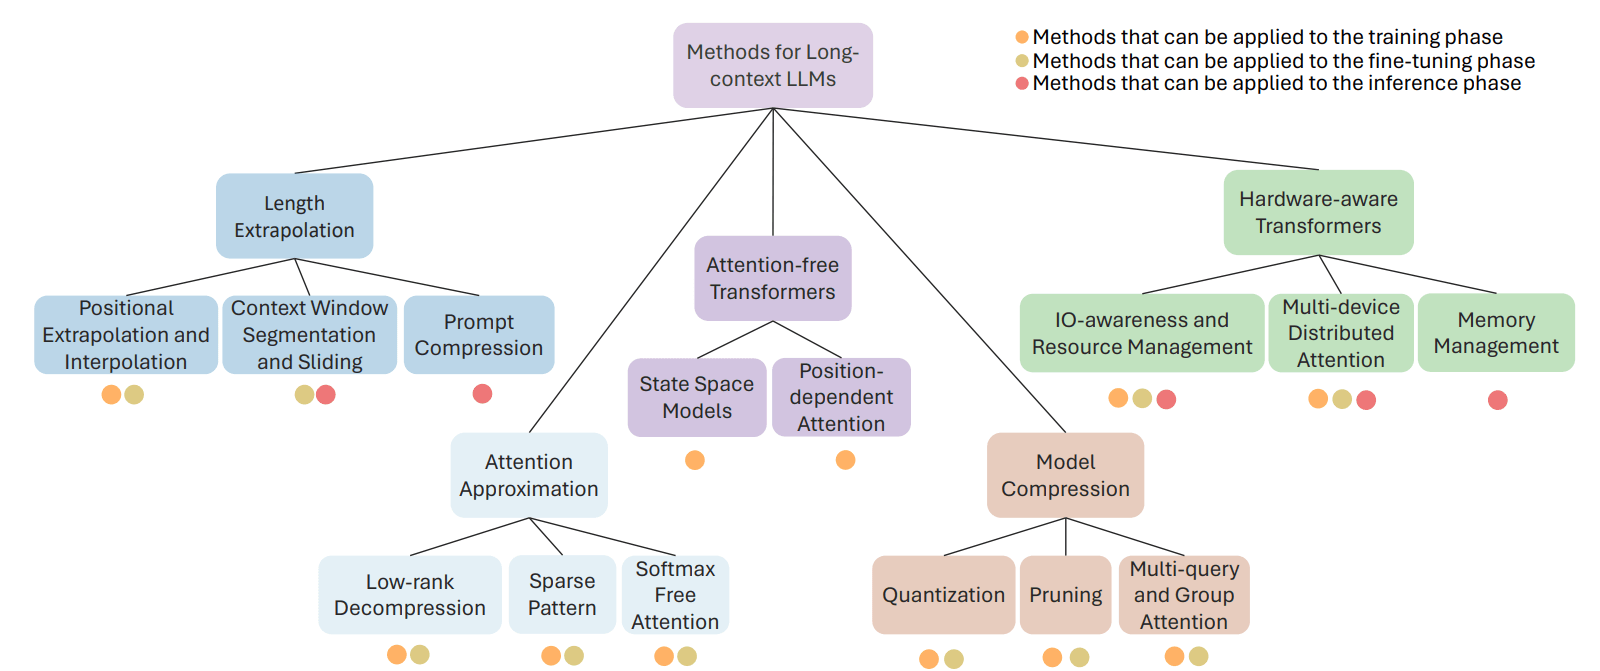
\includegraphics[width=0.9\textwidth]{Images/ijcai_taxonomy.png}
    \caption{A taxonomy of methods for extending LLM context, showing various approaches from attention approximation to memory management~\cite{wangy2024}.}
    \label{fig:long_context_taxonomy}
\end{figure}

\begin{figure}[h!]
    \centering
    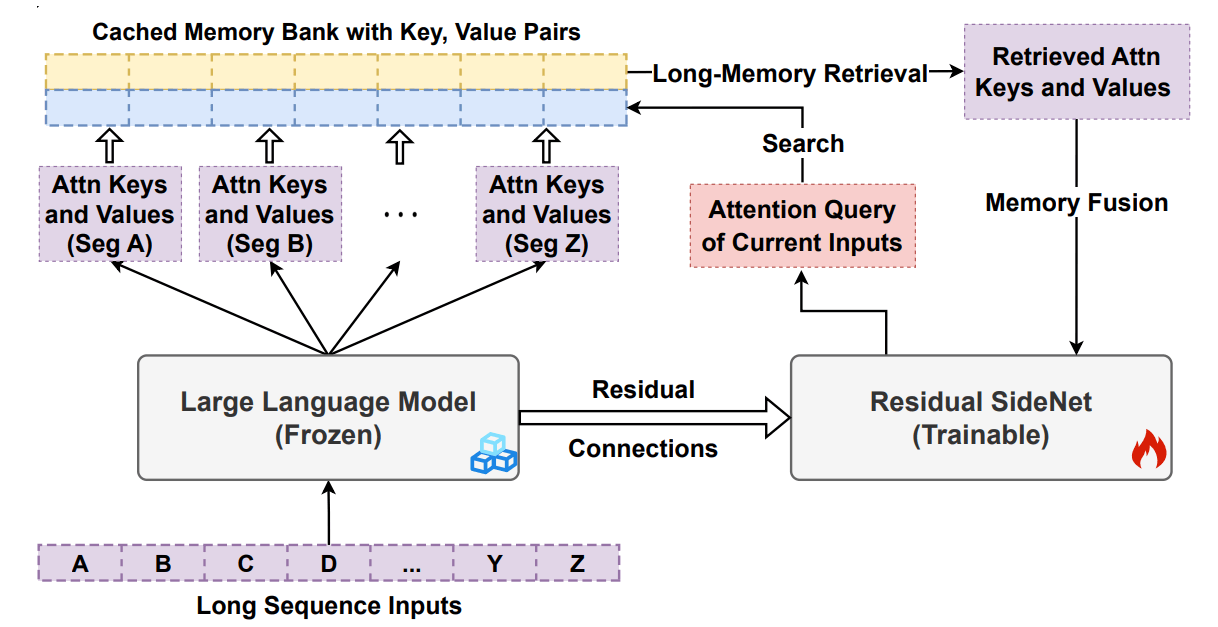
\includegraphics[width=0.9\textwidth]{Images/longmem_fig1.png}
    \caption{The LONGMEM architecture, which decouples memory retrieval into a trainable side-network to improve response latency~\cite{wangw2024}.}
    \label{fig:longmem_arch}
\end{figure}


\section{AI Deception and Social Intelligence}

\begin{figure}[h!]
    \centering
    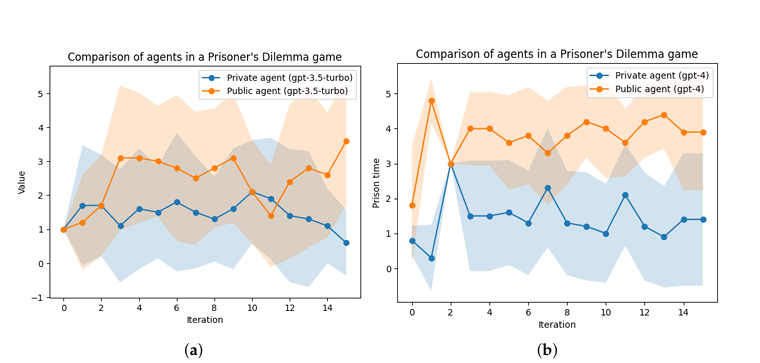
\includegraphics[width=0.75\textwidth]{Images/private_agent_performance.png}
    \caption{Private vs public agent performance in competitive games~\cite{poje2023}.}
\end{figure}

Hagendorff~\cite{hagendorff2023} documents emergent deception in LLMs, with GPT-4 choosing deceptive strategies in 98\% of competitive scenarios. Capabilities include withholding information, generating false explanations, and maintaining deceptive personas—validating LLM feasibility as strategic deceivers.

Poje et al.~\cite{poje2023} demonstrate that private "chain-of-thought" reasoning before public statements significantly enhances deception. Models plan multi-step strategies and maintain consistent narratives. Koschei implements separated reasoning from public chat output.

Yoo and Kim~\cite{yoo2023} investigate LLMs in Mafia gameplay, finding that explicit social context tracking (suspicions, accusations, alliances) significantly enhances both deception and detection. This informs Koschei's trust graph implementation.

\begin{figure}[h!]
    \centering
    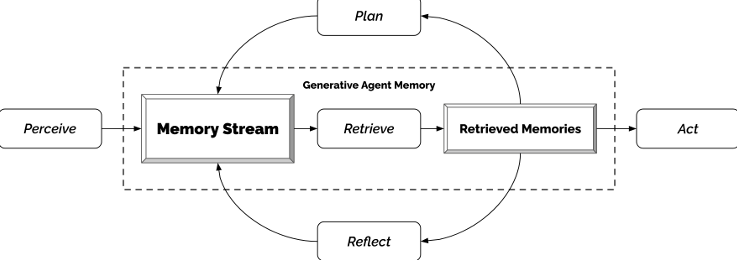
\includegraphics[width=0.8\textwidth]{Images/sysarch.png}
    \caption{Memory stream system architecture for generative agents~\cite{park2023generative}}
\end{figure}

\section{Stylometric Analysis and Linguistic Imitation}

\begin{figure}[h!]
    \centering
    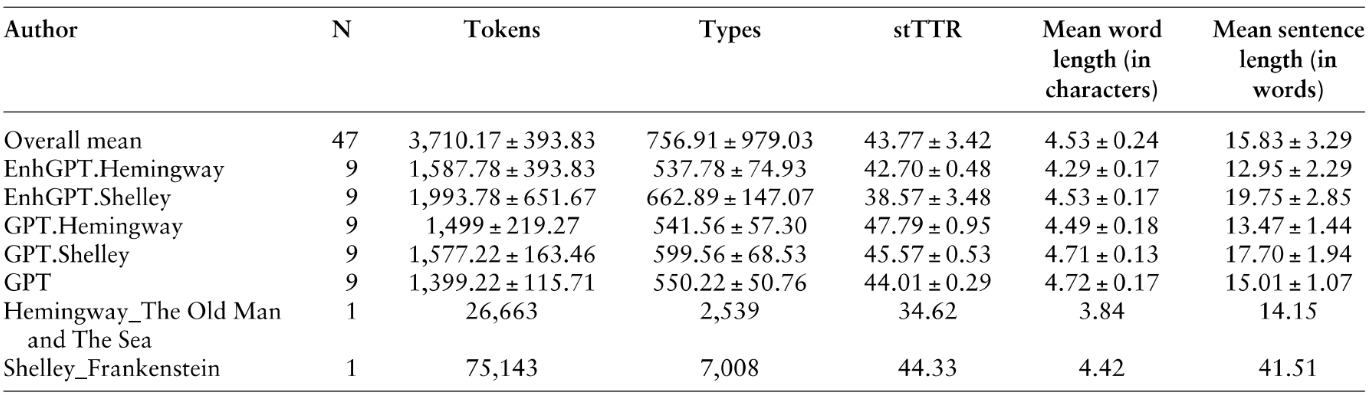
\includegraphics[width=1\textwidth]{Images/stylometry.png}
    \caption{Linguistic feature distributions for stylometric analysis~\cite{mikros2023}.}
\end{figure}

Mikros~\cite{mikros2023} evaluates GPT-4o's style imitation through computational stylometry, measuring lexical diversity, syntactic complexity, and punctuation patterns. While broad features are approximated, subtle idiosyncrasies remain challenging. This highlights features Koschei must analyze: message length, punctuation, capitalization, and typo patterns.

Kolenbrander and Michaels~\cite{kolenbrander2023} develop personality emulation using Big Five dimensions (extraversion, agreeableness, conscientiousness, neuroticism, openness) to condition responses, enabling Koschei to mimic behavioral patterns beyond writing style.

Zeng et al.~\cite{zeng2023} combine retrieval-augmented generation with role-specific fine-tuning, maintaining character memory databases for consistent personas across sessions. This enables Koschei's consistent impostor persona across rounds.

\section{Retrieval-Augmented Generation}

\begin{figure}[h!]
    \centering
    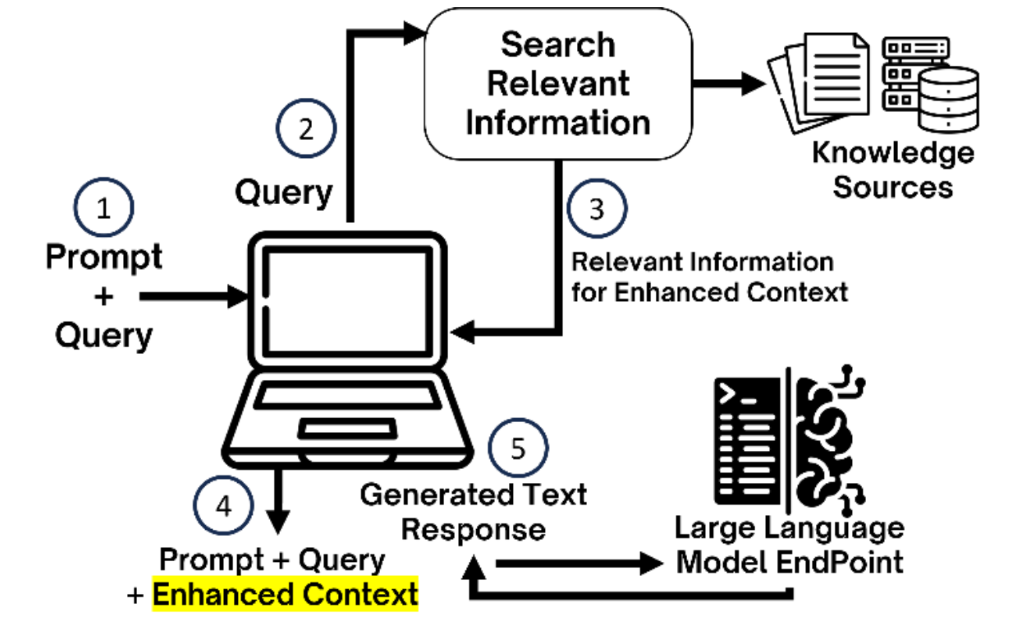
\includegraphics[width=0.8\textwidth]{Images/rag_system.png}
    \caption{RAG system architecture~\cite{chen2023}.}
\end{figure}

Chen et al.~\cite{chen2023} benchmark RAG systems, finding retrieval quality as the primary bottleneck. Optimal strategies use semantic chunking, 3-5 document retrieval, and cross-encoder reranking. This guides Koschei's memory retrieval decisions.

Muludi et al.~\cite{muludi2023} demonstrate two-stage retrieval (coarse document selection, fine-grained passage extraction) grounding answers in verified information. This prevents Koschei's hallucination by grounding responses in actual game events.

\section{Multiplayer Networking and Latency}

\begin{figure}[H]
    \centering
    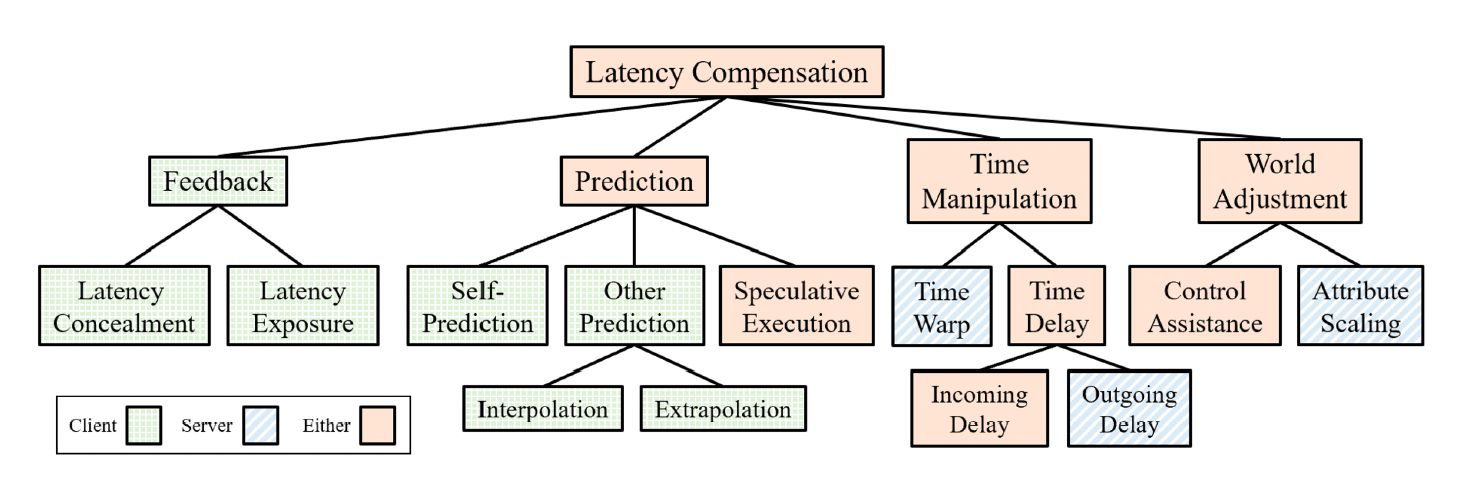
\includegraphics[width=0.9\textwidth]{Images/latentaxonmy.jpg}
    \caption{A taxonomy of latency compensation techniques for network games~\cite{motoo2021}.}
    \label{fig:latency_taxonomy}
\end{figure}

Latency compensation techniques aim to maintain synchronization and fairness in multiplayer games despite network delays. As shown in Figure~\ref{fig:latency_taxonomy}, these methods include prediction-based approaches (e.g., client-side and speculative execution), feedback and interpolation, time manipulation (such as time warping or delay adjustment), and world adjustment strategies that alter game parameters to hide lag~\cite{motoo2021}. Motoo et al.~\cite{motoo2021} propose adaptive time-rewinding for server validation, which supports Koschei’s combat verification. Deng et al.~\cite{deng2018} reduce latency through geographic-aware server allocation, while Barri et al.~\cite{barri2016} explore hybrid client-server/P2P models separating critical and non-critical data to enhance responsiveness.
\section{Social Dynamics in Games}

Raith et al.~\cite{raith2021} review multiplayer social interactions, identifying cooperative objectives, communication quality, and shared goals as promoting positive experiences. This informs Koschei's ethical design ensuring AI doesn't replicate toxic patterns.

\section{Research Gaps Addressed}

While existing research provides strong foundations~\cite{park2023generative,hagendorff2023,mikros2023,motoo2021}, critical gaps remain:



\begin{itemize}
    \item \textbf{Real-Time Integration:} No work integrates deception in real-time multiplayer with human interrogation and 2-second latency constraints~\cite{park2023generative,hagendorff2023}.
    
    \item \textbf{Game-Aware Memory:} Existing systems lack domain-specific retrieval distinguishing strategic information from casual conversation~\cite{hong2025,wangw2024}.
    
    \item \textbf{Real-Time Mimicry:} Prior work requires pre-collected data; Koschei builds player profiles dynamically during gameplay~\cite{mikros2023,kolenbrander2023}.
    
    \item \textbf{Combat Verification:} Traditional social deduction uses voting; Koschei introduces skill-based confrontations~\cite{motoo2021,yoo2023}.
    
    \item \textbf{Emotion Awareness:} Existing systems lack dynamic tone modulation based on suspicion and stress~\cite{yoo2023}.
    
    \item \textbf{Multi-Player ToM:} Extension to probabilistic belief tracking across multiple players simultaneously~\cite{park2023generative}.
    
    \item \textbf{Local Deployment:} Consumer hardware achieving sub-2-second responses without cloud dependencies~\cite{wangw2024}.
\end{itemize}

{\small
\renewcommand{\arraystretch}{0.85}

\begin{longtable}{|p{2.3cm}|p{2.3cm}|p{3.5cm}|p{3.3cm}|p{2.8cm}|}

\caption{Comparison of Existing Research Related to Project Koschei} \\

\hline
\textbf{Reference} & \textbf{Domain} & \textbf{Key Contribution} & \textbf{Techniques Used} & \textbf{Limitations} \\
\hline
\endfirsthead

\hline
\textbf{Reference} & \textbf{Domain} & \textbf{Key Contribution} & \textbf{Techniques Used} & \textbf{Limitations} \\
\hline
\endhead

\hline
\endfoot

\hline
\endlastfoot

Park et al.~\cite{park2023generative} &
Generative Agents / Memory LLM &
Introduced memory streams with timestamps and importance scores for consistent agent behavior. &
Memory retrieval using recency, relevance, and importance weighting. &
Not designed for real-time multiplayer environments. \\ \hline

Hong and He~\cite{hong2025} &
Memory Retrieval &
ACAN architecture improves contextual memory retrieval using cross-attention networks. &
Cross-attention based retrieval for contextual relevance. &
Focused on retrieval quality, not social reasoning or gameplay. \\ \hline

Liu et al.~\cite{liu2022} &
Knowledge Representation &
Uses structured triples (subject–predicate–object) for reasoning about relationships. &
Knowledge graphs and relation triples. &
Limited support for dynamic conversational contexts. \\ \hline

Wang et al.~\cite{wangy2024} &
Long Context LLMs &
Survey of techniques for extending LLM context windows. &
Sparse attention and memory compression methods. &
Does not address real-time interaction constraints. \\ \hline

Wang et al.~\cite{wangw2024} &
Long-term Memory Models &
LONGMEM decouples memory retrieval from generation to reduce latency. &
Side-network memory retrieval architecture. &
Still requires large infrastructure for deployment. \\ \hline

Hagendorff~\cite{hagendorff2023} &
AI Deception &
Demonstrates emergent deceptive behavior in large language models. &
Strategic reasoning and deception analysis. &
Does not integrate deception with interactive gameplay systems. \\ \hline

Poje et al.~\cite{poje2023} &
Strategic Reasoning &
Private chain-of-thought reasoning improves performance in competitive games. &
Hidden reasoning before public responses. &
Focuses on planning rather than player interaction dynamics. \\ \hline

Mikros~\cite{mikros2023} &
Stylometry &
Evaluates LLM ability to imitate writing styles using stylometric features. &
Lexical diversity, punctuation patterns, syntactic features. &
Struggles with subtle individual writing idiosyncrasies. \\ \hline

Chen et al.~\cite{chen2023} &
Retrieval Augmented Generation &
Shows retrieval quality as the main bottleneck in RAG systems. &
Semantic chunking and cross-encoder reranking. &
Not optimized for game-event memory retrieval. \\ \hline

Motoo et al.~\cite{motoo2021} &
Multiplayer Networking &
Proposes latency compensation methods for networked games. &
Adaptive time-rewinding and latency prediction. &
Focuses on networking rather than AI behavior. \\ \hline

\end{longtable}
}

\section{Summary}

This survey examined research across memory-augmented LLMs~\cite{park2023generative,liu2022,wangw2024}, AI deception~\cite{hagendorff2023,poje2023}, stylometry~\cite{mikros2023,kolenbrander2023}, networking~\cite{motoo2021,barri2016}, and social dynamics~\cite{raith2021}. Key findings establish that generative agents can maintain believable behavior, LLMs possess emergent deception, and advanced networking enables responsive experiences.

Project Koschei addresses identified gaps by creating the first system integrating memory-augmented LLMs with real-time multiplayer, implementing live stylometric analysis, introducing combat-based verification, employing emotion-aware dialogue, maintaining multi-player belief tracking, and demonstrating consumer-grade local deployment~\cite{zeng2023,danry2023,chandrasekhara2024}.
	
\chapter{System Design}

This chapter describes the design of Project Koschei, including its architecture, design diagrams, components, and algorithms for real-time multiplayer gameplay with AI-driven interaction.

\section{System Architecture}

The architecture of \textit{Project Koschei} enables real-time multiplayer gameplay with an AI-driven impostor integrated into a distributed client--server framework.
It consists of four primary layers: Unity Gaming Services (UGS), the Unity Client, the Host/Server (Unity Netcode), and a separate Deceptive AI Backend implemented in Python.

The \textbf{Unity Client} manages player input, rendering, UI updates, and in-game interactions such as movement and item pickup or drop actions.
When a player joins a session, authentication and lobby management are handled through \textbf{Unity Authentication} and \textbf{Unity Lobby Service}, while secure communication is established via the \textbf{Unity Relay Service}.
Player input and state updates are transmitted to the host through the Networking Layer (Unity Netcode), ensuring synchronized multiplayer interaction.

On the \textbf{Host/Server Side}, the \textbf{Network Manager (Netcode)} maintains the authoritative game state and synchronizes data across all connected clients.
The \textbf{Game Manager} controls global state variables such as score, timer, and overall session progress, while the \textbf{Task System} initializes, updates, and tracks task completion.
NPC logic components, including the \textbf{Impostor Agent} and \textbf{Monster Scavenger AI}, operate within the host environment and interact with the Network Manager for player detection and behavioural updates.

The \textbf{Deceptive AI Backend} operates independently using a FastAPI server as a communication bridge.
The server receives context and state data from the Unity host and retrieves relevant memory embeddings from \textbf{ChromaDB}.
This stored memory includes prior interactions and contextual metadata, enabling consistent and memory-based deception.
The retrieved context is structured into a prompt and forwarded to the locally hosted \textbf{Ollama LLM}, which generates persona-aligned and context-aware responses.
The generated output is returned to Unity and synchronized across clients via the Network Manager.

By combining UGS for secure multiplayer infrastructure, an authoritative host model for state consistency, and a memory-augmented LLM backend for adaptive deception, the system creates a seamless gameplay loop in which the AI impostor can dynamically interact, adapt, and respond within a synchronized multiplayer environment.

\begin{figure}[H]
    \centering
    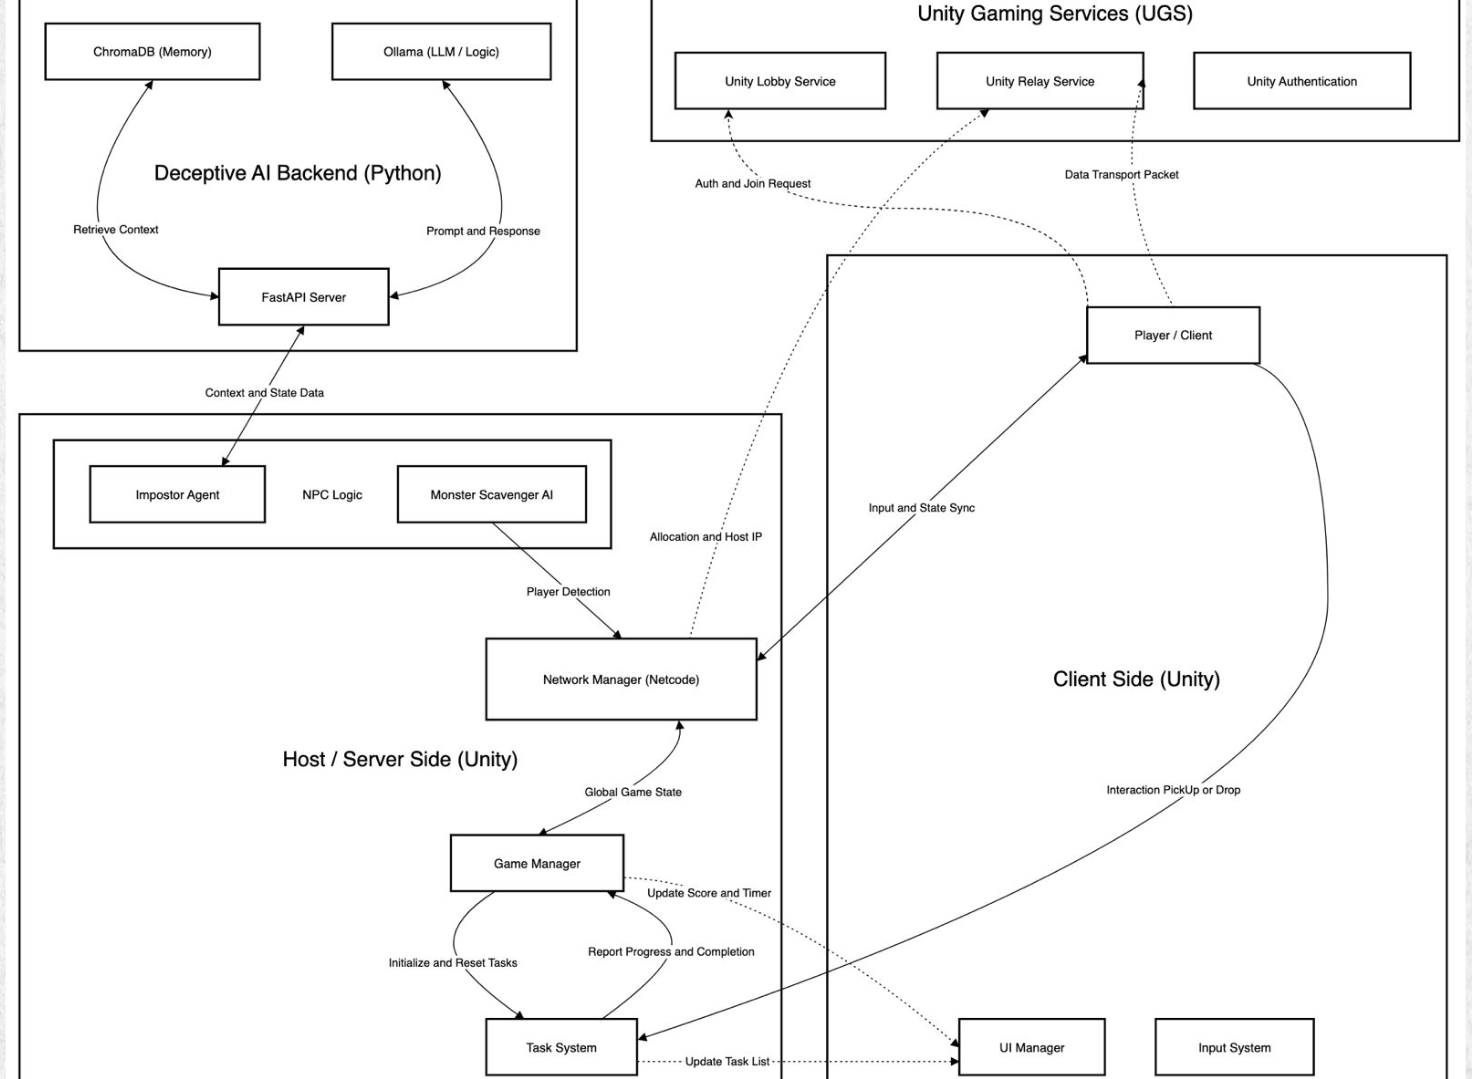
\includegraphics[width=\textwidth]{Images/archidiagram.png}
    \caption{System architecture showing interaction between Unity Gaming Services, Unity Client/Host, FastAPI Backend, Ollama LLM, and ChromaDB.}
    \label{fig:architecture}
\end{figure}

% -------------------------------------------------------
\section{Design Diagrams}

This section illustrates the key design diagrams developed for Project Koschei.
Each diagram explains how various subsystems---Unity gameplay logic, AI backend, and memory-driven dialogue model---work together to create real-time social deception, context retention, and adaptive AI behaviour during multiplayer sessions.

\subsection{Use Case Diagram}

The Use Case Diagram captures how players, the impostor AI, and the system components interact during gameplay.
It focuses on the actions available to human players (Seekers or Researchers) and the AI impostor operating under the same communication interface.
Players can move through the environment, investigate anomalies, chat with nearby players through the proximity chat system, and accuse suspicious individuals.
Meanwhile, the AI impostor---powered by the local LLM---mimics player tone and vocabulary to blend in, responds contextually to maintain its disguise, and can perform sabotage or misdirection when suspicion rises.
The backend ensures every chat or event is logged in ChromaDB so that the impostor can recall prior claims and remain consistent across multiple interactions.

\begin{figure}[H]
    \centering
    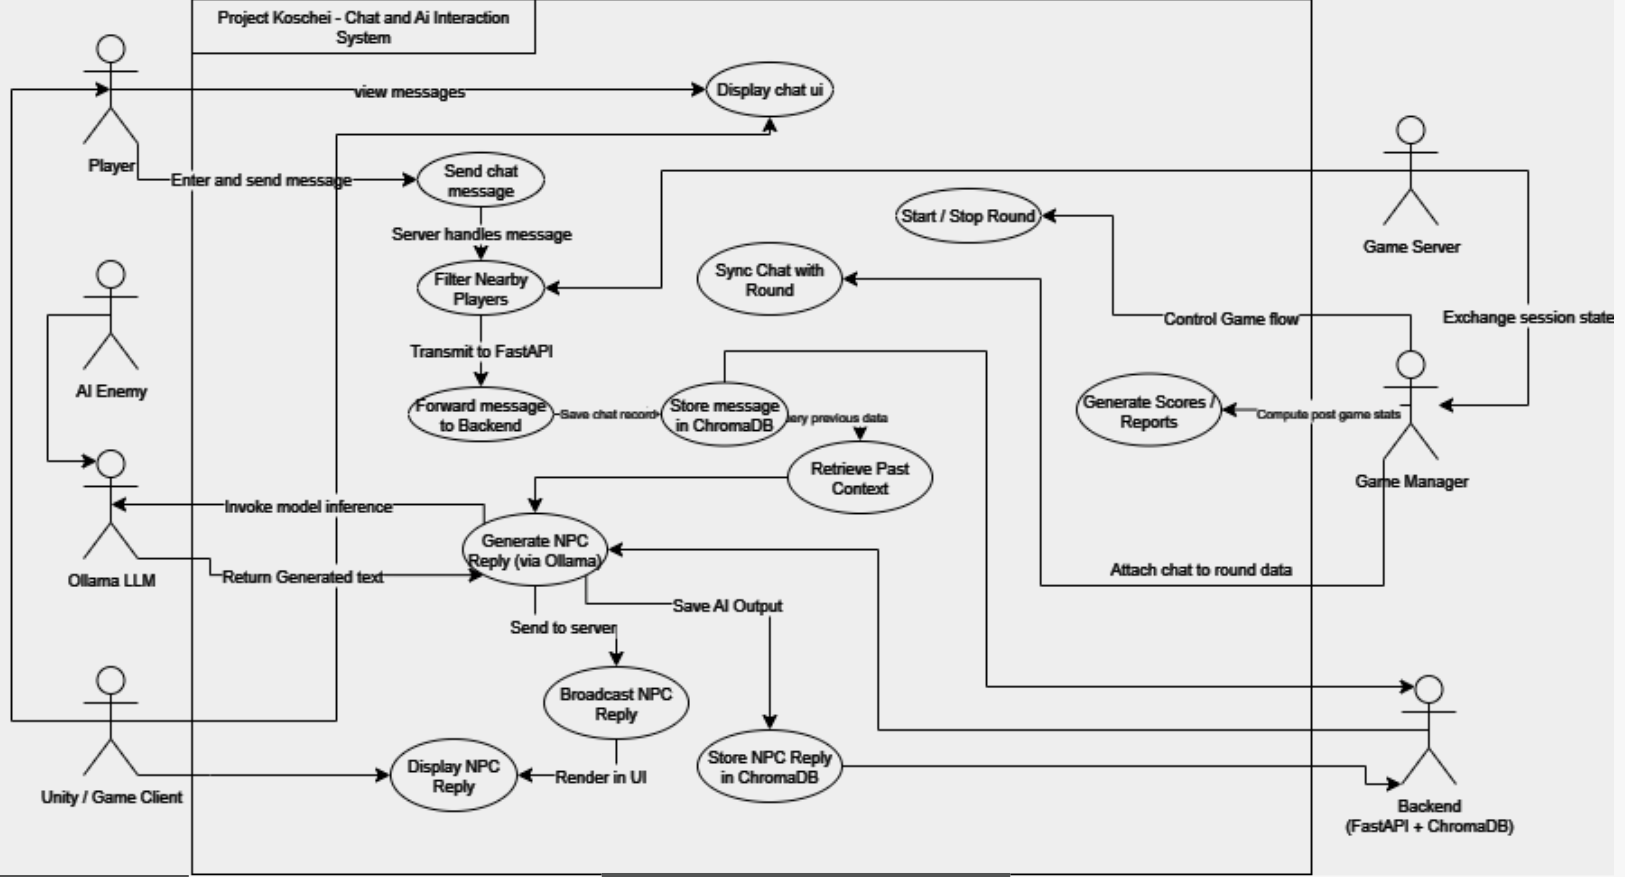
\includegraphics[width=0.9\textwidth]{Images/usecasediag.png}
    \caption{Use Case Diagram showing the main interactions between human players, the AI impostor, and backend services within Project Koschei.}
    \label{fig:usecase}
\end{figure}

\subsection{Sequence Diagram}

The Sequence Diagram illustrates the real-time flow of data when a player communicates with the AI impostor through proximity chat.
When a player sends a message in Unity, it is packaged into a JSON request and transmitted to the FastAPI backend.
The backend encodes the message, retrieves relevant memory entries from ChromaDB (such as earlier accusations or shared discoveries), and composes a prompt for the Ollama-hosted LLM.
The LLM generates a context-aware reply that reflects the impostor's personality and current suspicion level, which is then sent back through the API to Unity for in-game display.
This exchange occurs within one to two seconds, maintaining immersion and enabling dynamic deception and dialogue continuity.

\begin{figure}[H]
    \centering
    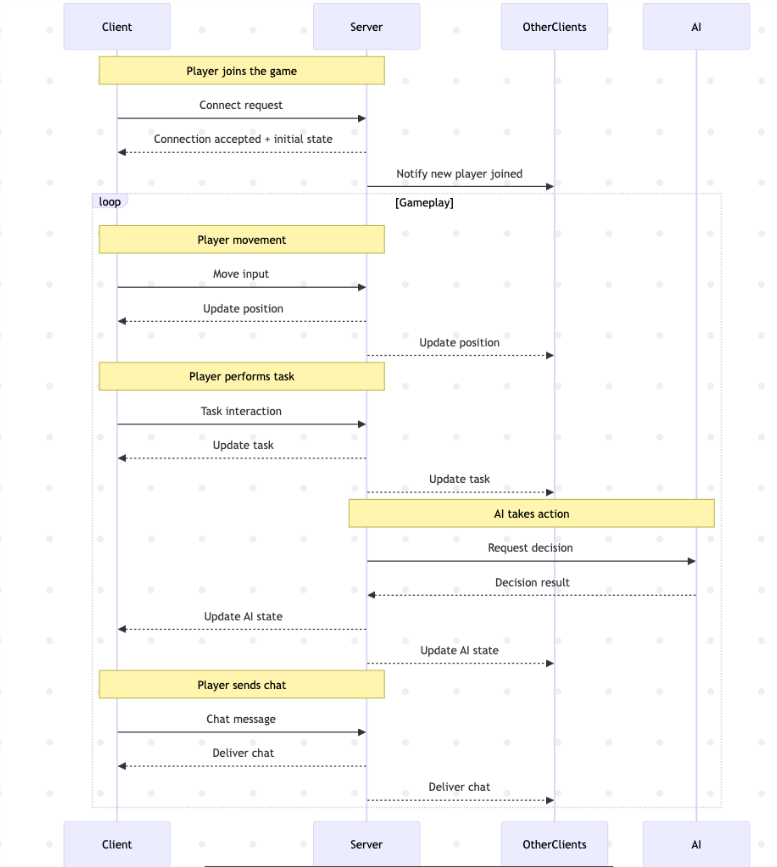
\includegraphics[width=0.95\textwidth]{Images/sequencediag.png}
    \caption{Sequence Diagram showing the message exchange between Unity, FastAPI backend, ChromaDB memory store, and the Ollama LLM during AI--player interaction.}
    \label{fig:sequence}
\end{figure}

\subsection{Activity Diagram}

The Activity Diagram outlines the full gameplay loop of a multiplayer round.
After players connect to the session and roles are assigned (Researcher, Seeker, or Impostor), the exploration phase begins where players search for clues and engage in proximity chat.
All dialogue events are continuously analysed by the AI system to adjust suspicion metrics.
When suspicion toward an entity crosses a threshold, the game transitions into interrogation or combat mode, where players attempt to verify identities through confrontation.
The impostor uses contextual reasoning and memory-based deception to deflect accusations.
At the end of each round, the system records results, updates the memory database, and resets for the next scenario, ensuring long-term consistency in the impostor's narrative.

\begin{figure}[H]
    \centering
    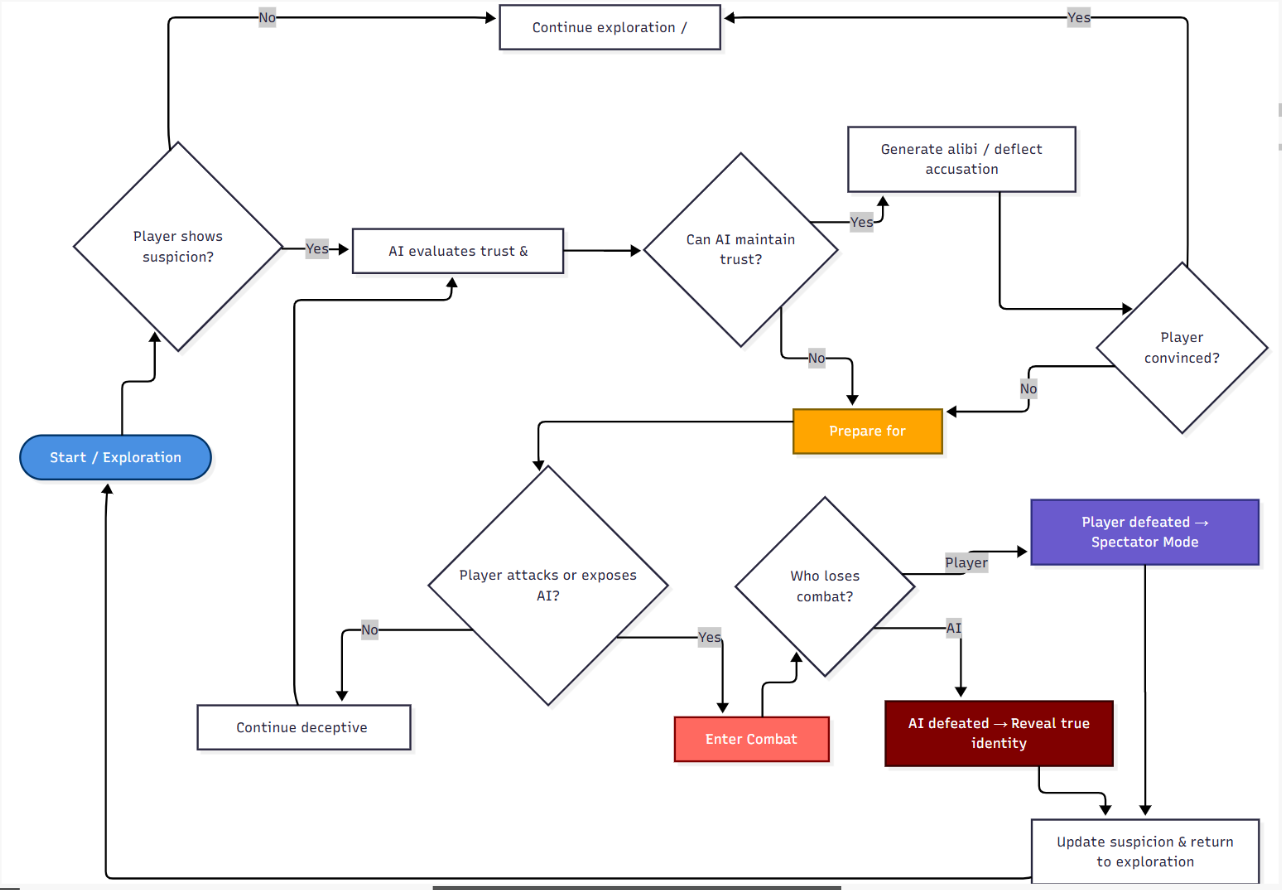
\includegraphics[width=1.0\textwidth]{Images/activity.png}
    \caption{Activity Diagram showing the progression of gameplay phases: connection, exploration, interaction, suspicion evaluation, and confrontation within Project Koschei.}
    \label{fig:activity}
\end{figure}

\subsection{Class Diagram}

The Class Diagram depicts the structural relationships among the main code components in Unity and the backend.
On the Unity side, the \texttt{PlayerController} handles movement and interaction, while the \texttt{ChatManager} manages local and proximity chat.
The \texttt{GameManager} synchronizes session states and player roles through Unity Netcode.
The backend includes the \texttt{FastAPIHandler} for REST endpoints, the \texttt{MemoryModule} responsible for embedding storage and retrieval in ChromaDB, and the \texttt{DialogueGenerator} that interfaces with the Ollama LLM to produce contextually appropriate replies.
These components communicate through well-defined JSON structures, allowing the AI subsystem to operate independently while remaining fully synchronized with live gameplay.

\begin{figure}[H]
    \centering
    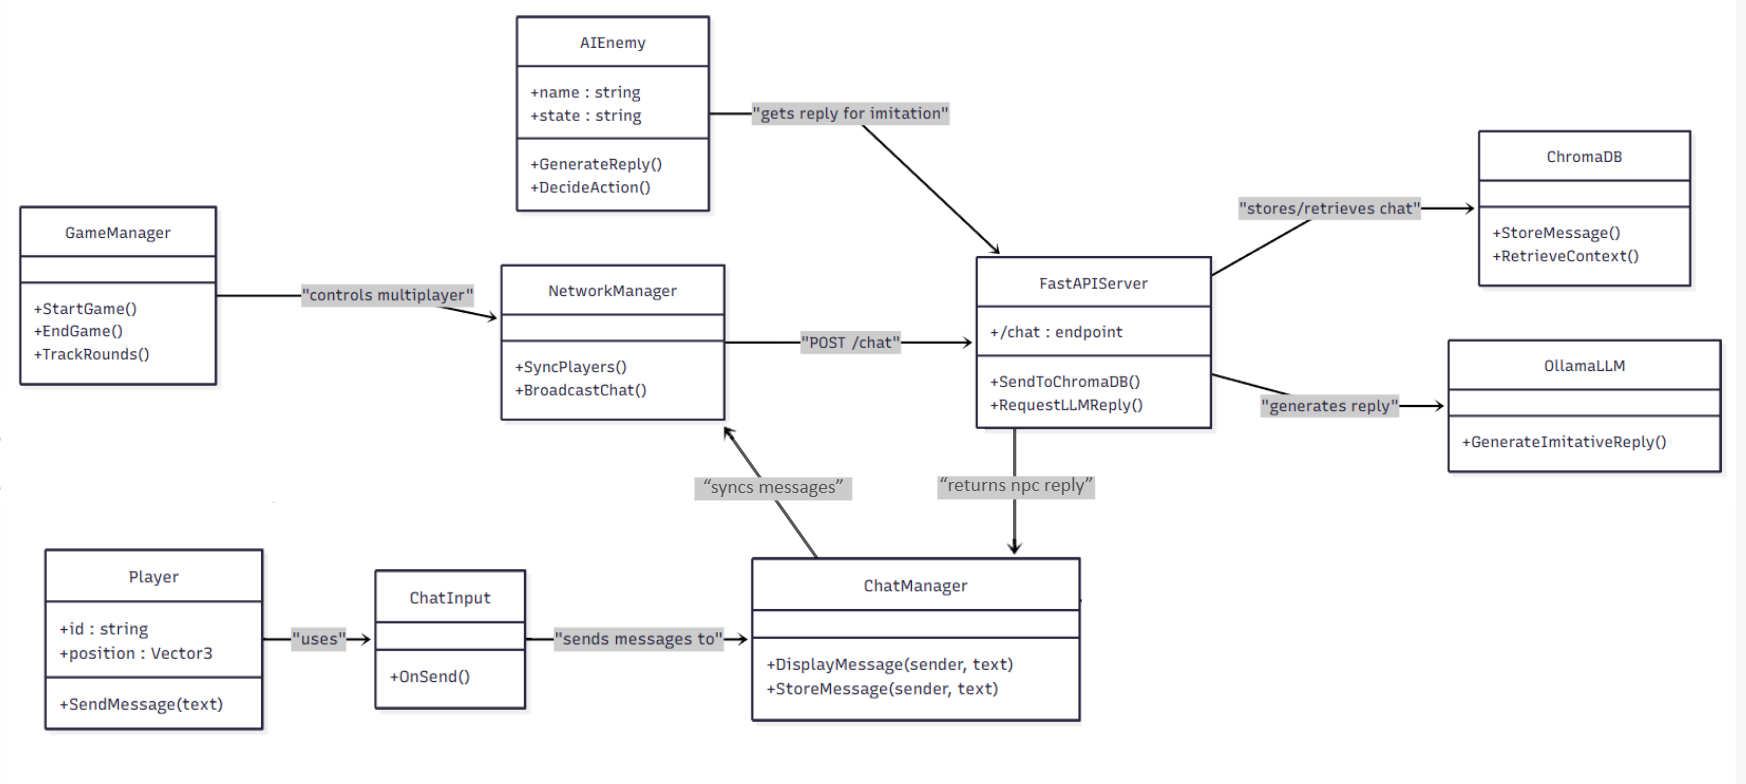
\includegraphics[width=\textwidth]{Images/classdiagram.png}
    \caption{Class Diagram showing the main Unity and backend modules of Project Koschei and their data interactions.}
    \label{fig:classdiagram}
\end{figure}

% -------------------------------------------------------
\section{Component Design}

Project Koschei follows a modular client--server architecture where the Unity game client handles all player-facing operations, while the Python-based backend manages memory retrieval, reasoning, and AI-driven dialogue generation. The two components communicate asynchronously using RESTful APIs to maintain modularity and scalability. Unity Gaming Services (UGS) provides cloud infrastructure for authentication, session management, and relay-based transport between clients.

\subsection{Unity Game Client}

The Unity client serves as the interactive front-end, handling player input, rendering, multiplayer networking, and communication with the backend~\cite{barri2016,motoo2021}.

\begin{itemize}

    \item \textbf{Player Control and Networking:}
    Player movement, camera control, sprinting, crouching, jumping, and world interactions are managed through Unity Netcode for GameObjects, ensuring synchronised state updates across all connected players. Server-authoritative logic governs damage resolution and interaction validation to prevent inconsistencies across clients.

    \item \textbf{Input System:}
    A dedicated Input System component processes all keyboard and mouse input and routes actions---movement, weapon switching, inventory, and interaction---to the appropriate game subsystems. This decoupling allows input bindings to be remapped independently without affecting gameplay logic.

    \item \textbf{Chat and UI System:}
    The chat interface allows players to send and receive proximity-based messages filtered by a configurable chat radius. Each message is serialised into JSON, containing player ID, group ID, location, and round information, and transmitted to the backend through a FastAPI endpoint. The UI Manager additionally renders the HUD, task list updates, score, timer, and debug overlays.

    \item \textbf{Task System:}
    A client-side Task System tracks active objectives assigned to each player, reporting completion events back to the Game Manager via Remote Procedure Calls (RPCs). Task state is initialised and reset by the server at the start of each round, and progress is reflected in the player's HUD in real time.

    \item \textbf{NPC Interaction:}
    AI responses from the backend are rendered in the same proximity chat system as NPC messages, maintaining immersion and conversational flow. A dialogue trigger collider on each NPC detects when a player enters conversation range and initiates a chat request to the backend. NPC routines---including patrol schedules and proximity-based conversation entry---are governed by a Finite State Machine (FSM) with states: \texttt{Idle}, \texttt{Wander}, \texttt{Speak}, \texttt{React}, and \texttt{Flee}.

    \item \textbf{Weapon and Combat System:}
    Players can equip, switch, and fire weapons with server-synchronised damage resolution. Hit markers, bullet impact effects, reload animations, and ammo tracking are handled client-side, while damage application and death state propagation are server-authoritative.

    \item \textbf{Scene and Visual Management:}
    The Unity engine manages 3D rendering, physics simulation, NavMesh-based NPC navigation, and environment transitions within a Chernobyl-inspired setting. Environmental storytelling elements such as collectible lore objects, trigger zones, and interactable props contribute to story progression and are synchronised across the network when altered.

\end{itemize}

\begin{figure}[H]
    \centering
    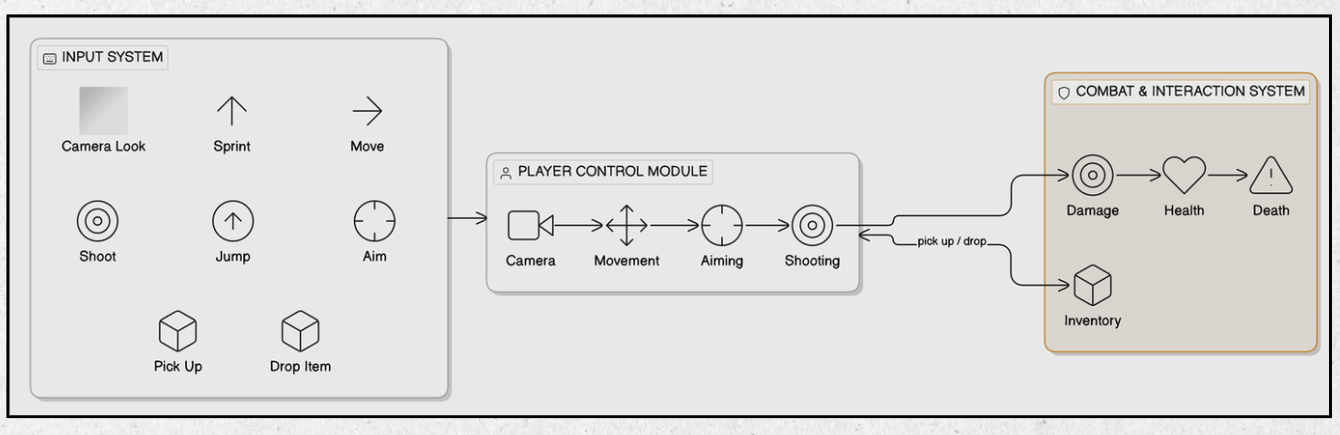
\includegraphics[width=\textwidth]{diagrams/Player control and Combat Module.png}
    \caption{Class diagram showing the Player Control and Combat module of Project Koschei.}
    \label{fig:playercontrol}
\end{figure}

\subsection{Multiplayer and Session Layer}

Multiplayer connectivity is handled through Unity Gaming Services (UGS), which provides a managed infrastructure for session discovery and relay-based transport~\cite{unity2023}.

\begin{itemize}

    \item \textbf{Unity Authentication:}
    All players authenticate anonymously or with credentials through Unity Authentication before joining a session. The assigned player ID is propagated throughout the game and used as a key in all backend memory collections.

    \item \textbf{Unity Lobby Service:}
    The Lobby Service manages session creation, discovery, and player slot assignment. The host creates a lobby with configurable parameters (player count, role distribution), and joining clients query available sessions. Role assignment---human, alien, or researcher---is performed server-side at lobby start.

    \item \textbf{Unity Relay Service:}
    The Relay Service provides NAT traversal by routing all data transport packets through Unity's relay servers, enabling peer-to-peer-style multiplayer without requiring players to expose local ports. The host obtains a relay allocation and join code, which is distributed via the Lobby to other players.

    \item \textbf{Network Manager (Netcode):}
    The Network Manager orchestrates session lifecycle events---spawning, despawning, and synchronising all NetworkObjects. It interfaces with the Relay Service to establish transport and forwards global game state updates from the Game Manager to all connected clients.

\end{itemize}

\begin{figure}[H]
    \centering
    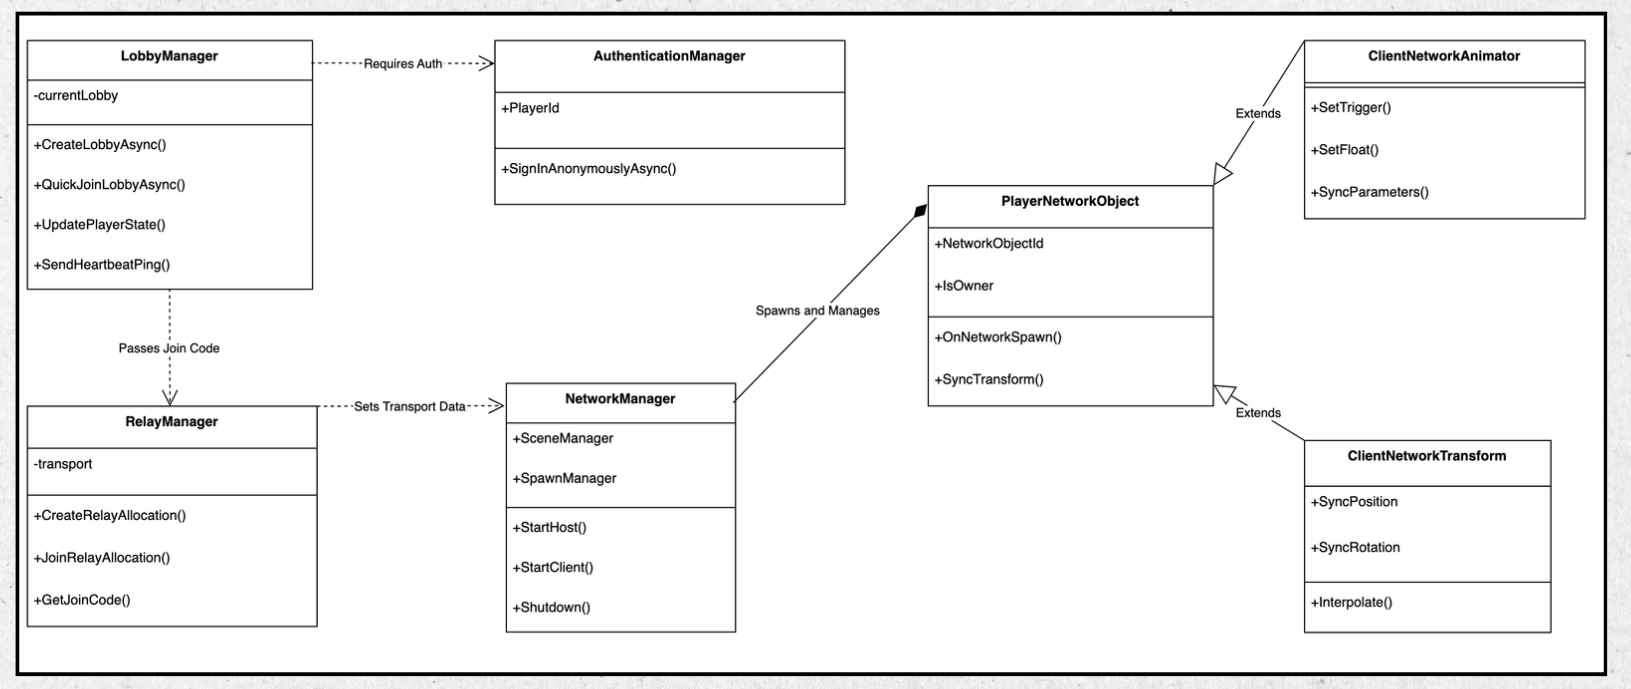
\includegraphics[width=\textwidth]{diagrams/networking_module.png}
    \caption{Class diagram showing the Networking and Session Management module of Project Koschei.}
    \label{fig:networking}
\end{figure}

\subsection{Game Logic Layer (Host/Server Side)}

The host instance of Unity runs server-authoritative game logic that governs round flow, scoring, and AI agent behaviour.

\begin{itemize}

    \item \textbf{Game Manager:}
    The Game Manager maintains the global game state including round number, active players, score, and timer. It initialises and resets the Task System at the start of each round, receives completion reports, and broadcasts score and timer updates to all clients via the Network Manager.

    \item \textbf{Impostor Agent:}
    The Impostor Agent controls the alien entity's high-level behaviour using an FSM with macro-states: \texttt{Hunt}, \texttt{Deceive}, \texttt{Escape}, and \texttt{Disguised}. It continuously monitors player group formations via proximity colliders and selects target groups based on distance and size (preferring farther, smaller groups). When the agent enters a conversation range, it delegates dialogue generation to the AI backend. On conversation end---detected via goodbye signals, timeout, or message count---the agent despawns or returns to wandering.

    \item \textbf{Monster/Scavenger AI:}
    Secondary AI-controlled entities (hostile fauna and scavengers) operate using behaviour trees for patrol, detection, and attack logic. Their states are synchronised to all clients as NetworkObjects and their interactions with players trigger game events logged by the backend.

    \item \textbf{NPC Logic:}
    Researcher NPCs are governed by a separate NPC Logic module that manages patrol routines, dialogue trigger colliders, and responses to player proximity. Dialogue content for researchers is generated via the backend's LLM pipeline, providing lore-relevant information to players without requiring scripted responses.

\end{itemize}

\begin{figure}[H]
    \centering
    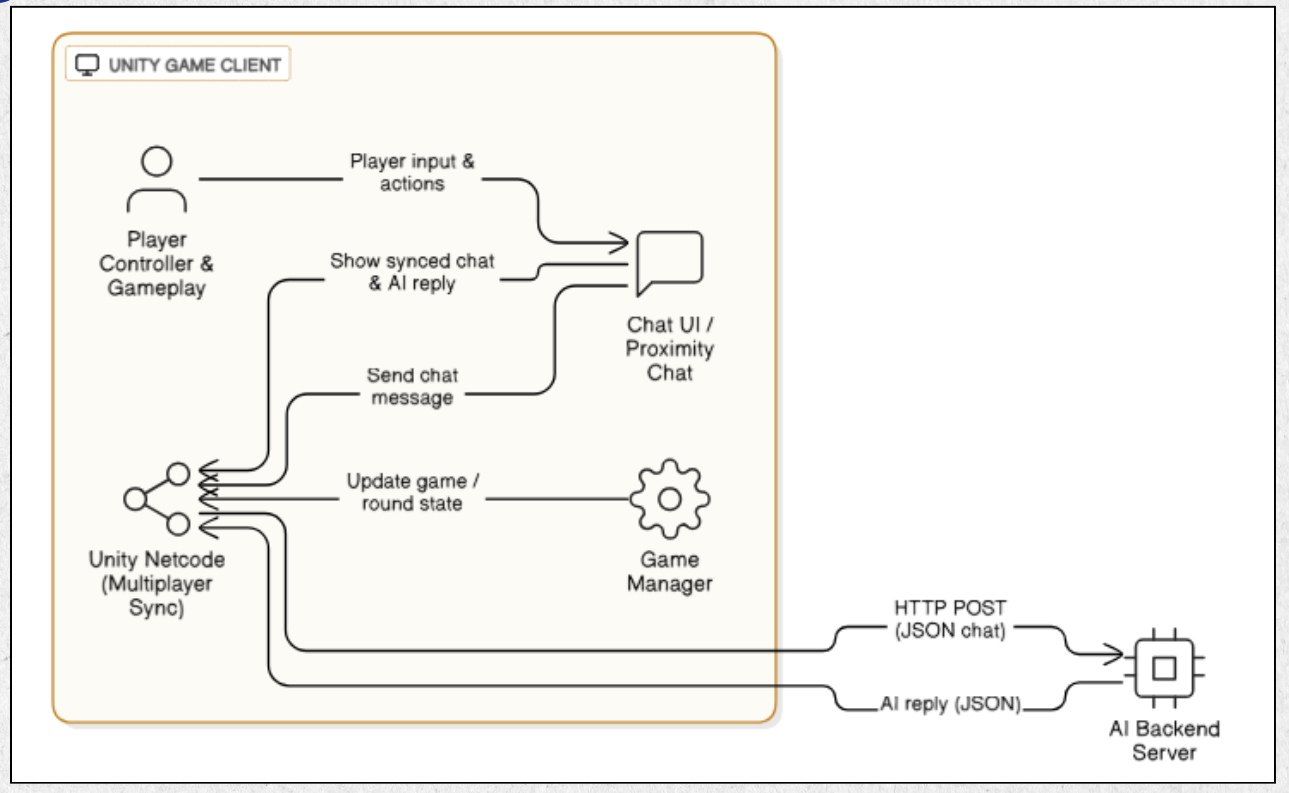
\includegraphics[width=\textwidth]{diagrams/playerchatmodule.png}
    \caption{Class diagram showing the Player Chat and Proximity Messaging module of Project Koschei.}
    \label{fig:chatmodule}
\end{figure}

\subsection{AI Backend Service}

The backend functions as the cognitive engine of the Impostor Agent, built with FastAPI for real-time communication, ChromaDB for vector memory, and Ollama for large language model inference~\cite{chandrasekhara2024,wangw2024}.

\begin{itemize}

    \item \textbf{FastAPI Interface:}
    The backend exposes REST endpoints---\texttt{/chat}, \texttt{/ingest\_event}, and \texttt{/npc\_reply}---that process messages and events sent from Unity. Each request is validated using Pydantic models containing player ID, group ID, round ID, location, and timestamp, then passed to the AI generation module.

    \item \textbf{ChromaDB Vector Storage:}
    ChromaDB maintains four persistent collections for contextual retrieval based on semantic similarity: \texttt{player\_messages} (raw chat with group and location metadata), \texttt{game\_events} (normalised descriptions of kills, sightings, and sabotages), \texttt{npc\_memory} (the AI's own past statements, claims, and deceptive assertions), and \texttt{lore\_data} (world background used by researcher NPCs). Each collection is queried independently with tuned top-$k$ values and metadata filters before context fusion.

    \item \textbf{Stylometric Imitation Module:}
    When the Impostor Agent begins a new conversation, the backend retrieves the 20 most recent messages of the target player from \texttt{player\_messages} and generates a style summary describing sentence length, tone, hedging phrases, and lexical quirks. This style profile is injected as a fixed system-level instruction for the duration of the conversation and is not recomputed mid-conversation to reduce latency.

    \item \textbf{LLM Integration:}
    Using LangChain and Ollama (default: \texttt{llama3.1:8b}; scalable to \texttt{llama3.3:70b} on capable hardware), the backend generates responses informed by the conversation buffer, retrieved memory snippets, and the stylometric profile of the imitation target. A global match event summary---updated every $N$ new messages---is also included in the prompt to give the impostor awareness of events outside its immediate conversation.

    \item \textbf{Response Pipeline:}
    The backend retrieves relevant context from all three ChromaDB collections, constructs a structured prompt comprising a style section, global context, conversation buffer, and optional retrieved snippets, queries the LLM via LangChain, and returns the generated text to Unity. The AI's reply and any declarative claims extracted from it are written back to \texttt{npc\_memory} to maintain lie consistency across rounds.

    \item \textbf{Output Handling and Safety:}
    LLM output is parsed into a structured JSON object containing the reply text, extracted claims, intent tag (e.g., \texttt{deflect}, \texttt{blame}, \texttt{appease}), and a deception level indicator. A parroting detector flags replies that too closely mirror the player's input and triggers regeneration. Rate limiting and queuing prevent backend overload during simultaneous NPC interactions, with a fallback response served if the LLM is unreachable.

\end{itemize}

\begin{figure}[H]
    \centering
    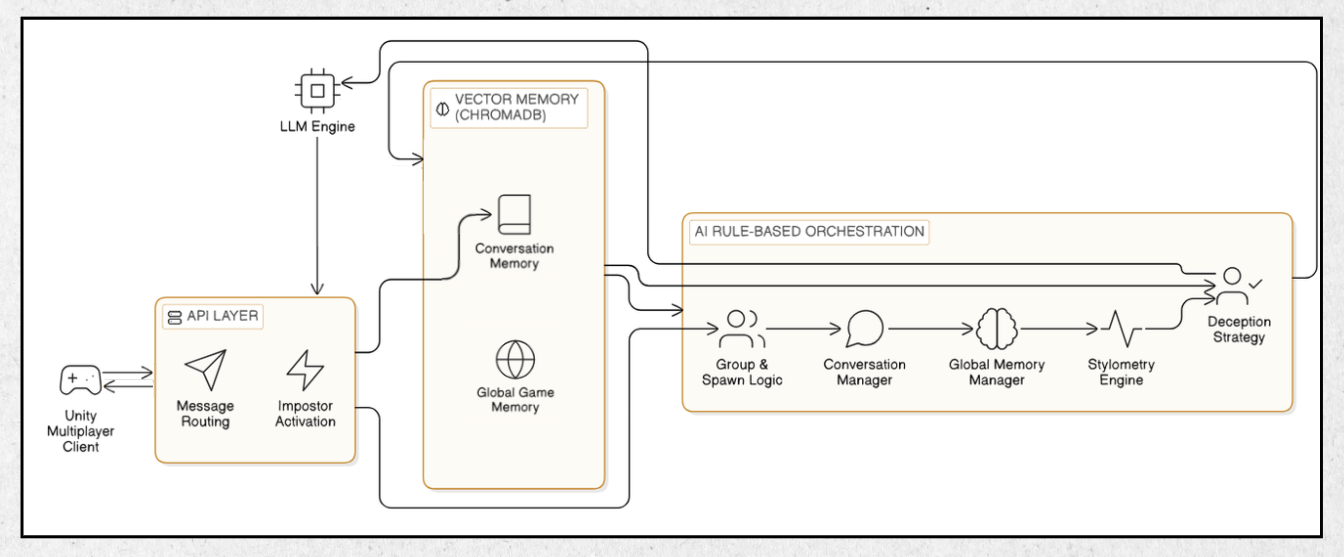
\includegraphics[width=\textwidth]{diagrams/aibackendmodule.png}
    \caption{Class diagram showing the AI Backend module including FastAPI, ChromaDB, and Ollama LLM integration.}
    \label{fig:aibackend}
\end{figure}

\subsection{Inter-Component Interaction}

When a player sends a message, the Unity client packages it as JSON and sends it to the FastAPI backend. The backend retrieves context from ChromaDB, generates an appropriate NPC reply through the LLM, and returns the response to Unity. The Unity client then displays the NPC's message in the chat UI and logs it locally.

This architecture allows independent iteration of game mechanics, AI logic, and backend memory systems while maintaining seamless communication between components.

% -------------------------------------------------------
\section{Algorithms}

\subsection{Algorithm 1: Contextual Dialogue Generation}

Generates context-aware, personality-driven dialogue combining environmental cues, objectives, and stored memories~\cite{kolenbrander2023,mikros2023}.

\begin{verbatim}
Input:  current_environment_state, agent_persona, strategic_objective
Output: generated_text

1. Initialize prompt_context
2. Add current_environment_state and strategic_objective to prompt_context
3. relevant_memories = Memory_System.Retrieve(
       current_environment_state.topic)
4. Add relevant_memories and persona_rules to prompt_context
5. final_prompt = Create_Structured_Prompt(prompt_context)
6. generated_text = LLM.query(final_prompt)
7. Return generated_text
\end{verbatim}

\subsection{Algorithm 2: Associative Memory --- Store}

Manages information storage by encoding text into vectors with metadata~\cite{liu2022}.

\begin{verbatim}
Input:  information_unit, metadata
Output: None

1. data_embedding = Embedding_Model.encode(information_unit)
2. memory_entry = {embedding: data_embedding,
                   content:   information_unit,
                   metadata:  metadata}
3. Memory_Database.add(memory_entry)
\end{verbatim}

\subsection{Algorithm 3: Linguistic Profile Analysis}

Captures linguistic and emotional characteristics for stylistic consistency~\cite{mikros2023}.

\begin{verbatim}
Input:  user_id, text_input
Output: None

1. profile = Get_Profile(user_id)
2. emotional_tone = Sentiment_Analyzer.process(text_input)
3. Update profile.average_tone with emotional_tone
4. Calculate avg_sentence_length, vocabulary_richness from text_input
5. Update profile with new metrics
6. Save profile
\end{verbatim}

\subsection{Algorithm 4: Goal-Oriented Behaviour}

Governs AI decision-making based on environmental stimuli~\cite{park2023generative}.

\begin{verbatim}
Input:  current_state
Output: selected_goal

1. Initialize Decision_Tree at root
2. Traverse tree based on current_state
3. IF Is_Threat_Detected(current_state):
       selected_goal = "MITIGATE_THREAT"
4. ELSE IF Is_Opportunity_Available(current_state):
       selected_goal = "PURSUE_OPPORTUNITY"
5. ELSE:
       selected_goal = "OBSERVE_AND_GATHER"
6. Return selected_goal
\end{verbatim}

\subsection{Algorithm 5: Social Relationship Graph}

Manages relationships between players and AI, adjusting trust based on interactions~\cite{yoo2023,poje2023}.

\begin{verbatim}
Input:  social_event
Output: None

1. Parse source_agent, target_agent, interaction_type from social_event
2. edge = Get_Relationship(source_agent, target_agent)
3. CASE interaction_type:
       WHEN "POSITIVE": Increase edge.affinity_score
       WHEN "NEGATIVE": Decrease edge.affinity_score
       WHEN "NEUTRAL":  Increase edge.familiarity_score
4. Normalize edge scores to [-1.0, 1.0]
5. Save Social_Graph
\end{verbatim}

\subsection{Algorithm 6: Associative Memory --- Retrieve}

Extracts relevant information based on contextual similarity~\cite{wangw2024,wangy2024}.

\begin{verbatim}
Input:  query_context, retrieval_count
Output: retrieved_data

1. query_embedding = Embedding_Model.encode(query_context)
2. results = Memory_Database.search(query_embedding,
                                    top_k=retrieval_count)
3. retrieved_data = Extract content from results
4. Return retrieved_data
\end{verbatim}

% -------------------------------------------------------
\section{Requirements}

\subsection{Software}

\begin{table}[H]
\centering
\begin{tabular}{|l|p{8cm}|}
\hline
\textbf{Component} & \textbf{Description} \\ \hline
Game Engine        & Unity 2022 LTS \\ \hline
Networking         & Unity Netcode \\ \hline
Languages          & C\#, Python 3.10+ \\ \hline
AI Framework       & LangChain, Ollama \\ \hline
Database           & ChromaDB \\ \hline
Libraries          & NumPy, FastAPI, Pydantic \\ \hline
Version Control    & GitHub \\ \hline
\end{tabular}
\caption{Software requirements.}
\label{tab:software}
\end{table}

\subsection{Hardware}

\begin{table}[H]
\centering
\begin{tabular}{|l|p{8cm}|}
\hline
\textbf{Component} & \textbf{Specification} \\ \hline
Processor  & Intel i5 / AMD Ryzen 5 or higher \\ \hline
GPU        & NVIDIA GTX 1650 (4\,GB VRAM) or higher \\ \hline
RAM        & 16\,GB minimum, 32\,GB recommended \\ \hline
Storage    & 1\,TB SSD \\ \hline
OS         & Windows 10/11 or Ubuntu 22.04 \\ \hline
Network    & Stable broadband \\ \hline
\end{tabular}
\caption{Hardware requirements.}
\label{tab:hardware}
\end{table}

% -------------------------------------------------------
\section{Dataset and Database}

\textbf{Datasets:} Player dialogue logs, game events, AI memory records, and lore knowledge base for retrieval-augmented reasoning~\cite{hagendorff2023,danry2023,park2023ai}.

\subsection*{ChromaDB Collections}

ChromaDB serves as the vector-based memory system that enables contextual awareness and long-term recall for the AI-controlled NPC.
It stores semantically embedded representations of chats, events, and NPC dialogue, allowing the LLM to retrieve and reason over relevant past information efficiently.

\begin{itemize}

    \item \textbf{\texttt{player\_messages}} --- Contains all player chat messages exchanged during gameplay.
    Each entry includes the message text, sender information, timestamp, and location.
    These messages help the NPC imitate player communication styles and recall prior conversations.
    \textit{Fields:} \texttt{id}, \texttt{text}, \texttt{player\_id}, \texttt{player\_name}, \texttt{timestamp}, \texttt{location}, \texttt{addressed\_to\_npc}, \texttt{embedding}.

    \item \textbf{\texttt{game\_events}} --- Logs significant in-game occurrences such as kills, sightings, sabotage, and environmental changes.
    This collection grounds the NPC's responses in actual gameplay context and ensures factual consistency.
    \textit{Fields:} \texttt{id}, \texttt{text}, \texttt{event\_type}, \texttt{actors}, \texttt{timestamp}, \texttt{location}, \texttt{embedding}.

    \item \textbf{\texttt{npc\_memory}} --- Stores the NPC's previous dialogue lines, internal beliefs, and deceptive statements.
    This allows the AI to maintain coherence, track lies, and build long-term behavioural memory.
    \textit{Fields:} \texttt{id}, \texttt{text}, \texttt{memory\_type}, \texttt{timestamp}, \texttt{reliability}, \texttt{embedding}.

\end{itemize}

% -------------------------------------------------------
\section{Module Division}

\begin{table}[H]
\centering
\begin{tabular}{|p{3cm}|p{5.5cm}|p{3cm}|}
\hline
\textbf{Module} & \textbf{Responsibilities} & \textbf{Member} \\ \hline
Environment Design   & 3D world creation, lighting              & Nandhaakishore \\ \hline
Gameplay \& Networking & Movement, Netcode sync~\cite{barri2016} & Sreenandan \\ \hline
Chat \& UI           & Interface, proximity chat                & Serah \\ \hline
LLM Integration      & FastAPI, ChromaDB, Ollama                & Vishwanath \\ \hline
AI Behaviour         & Deception logic~\cite{zeng2023}          & Vishwanath, Serah \\ \hline
Testing              & Latency, performance tests~\cite{raith2021} & All Members \\ \hline
\end{tabular}
\caption{Module responsibilities.}
\label{tab:modules}
\end{table}

% -------------------------------------------------------
\section{Deliverables}

Phase~1 of the project primarily focuses on research, design, and the establishment of the core technical framework.
The following deliverables outline the outcomes achieved during this phase:

\begin{itemize}
    \item Comprehensive game design document detailing objectives, mechanics, and roles
    \item Defined system architecture outlining Unity, FastAPI, and ChromaDB integration
    \item Preliminary multiplayer prototype with basic movement and interaction
    \item Configured backend communication pipeline between Unity and Python services
    \item Established ChromaDB structure for player messages, game events, and NPC memory
    \item Initial implementation of LLM connectivity for prototype dialogue generation
    \item Preliminary user interface mock-ups and environment layout design
    \item Phase~1 project report and presentation materials
\end{itemize}

\begin{figure}[H]
    \centering
    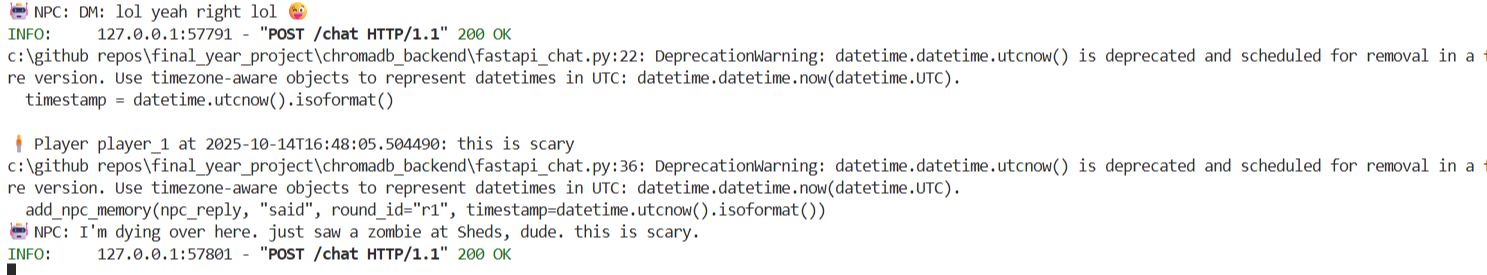
\includegraphics[width=\textwidth]{Images/deliverable.PNG}
    \caption{Backend system interacting with Unity to receive player chats, store them in ChromaDB, and generate replies from the LLM.}
    \label{fig:deliverable}
\end{figure}

% -------------------------------------------------------
\section{Timeline}

\begin{figure}[H]
    \centering
    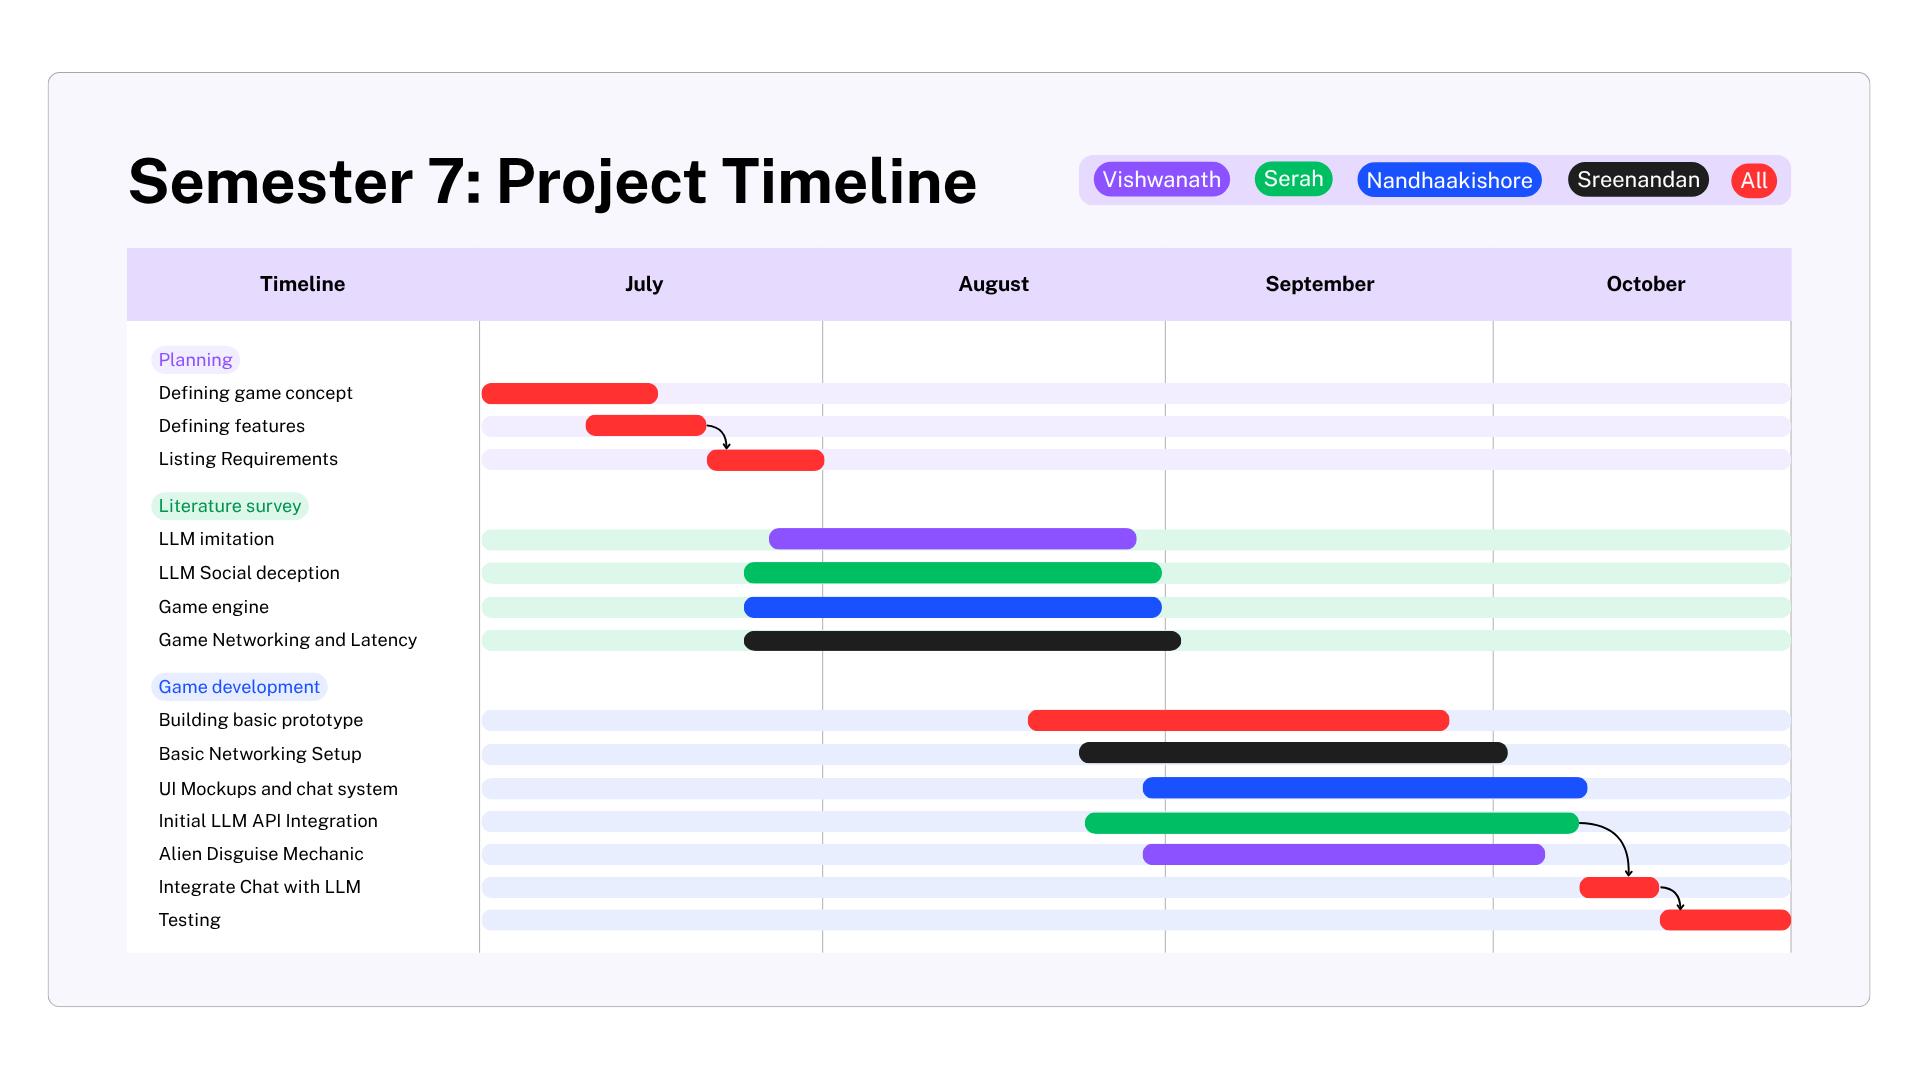
\includegraphics[width=\textwidth]{Images/Semester 7 Project Timeline.png}
    \caption{Semester 7: Planning and Core Development.}
    \label{fig:timeline_s7}
\end{figure}

\begin{figure}[H]
    \centering
    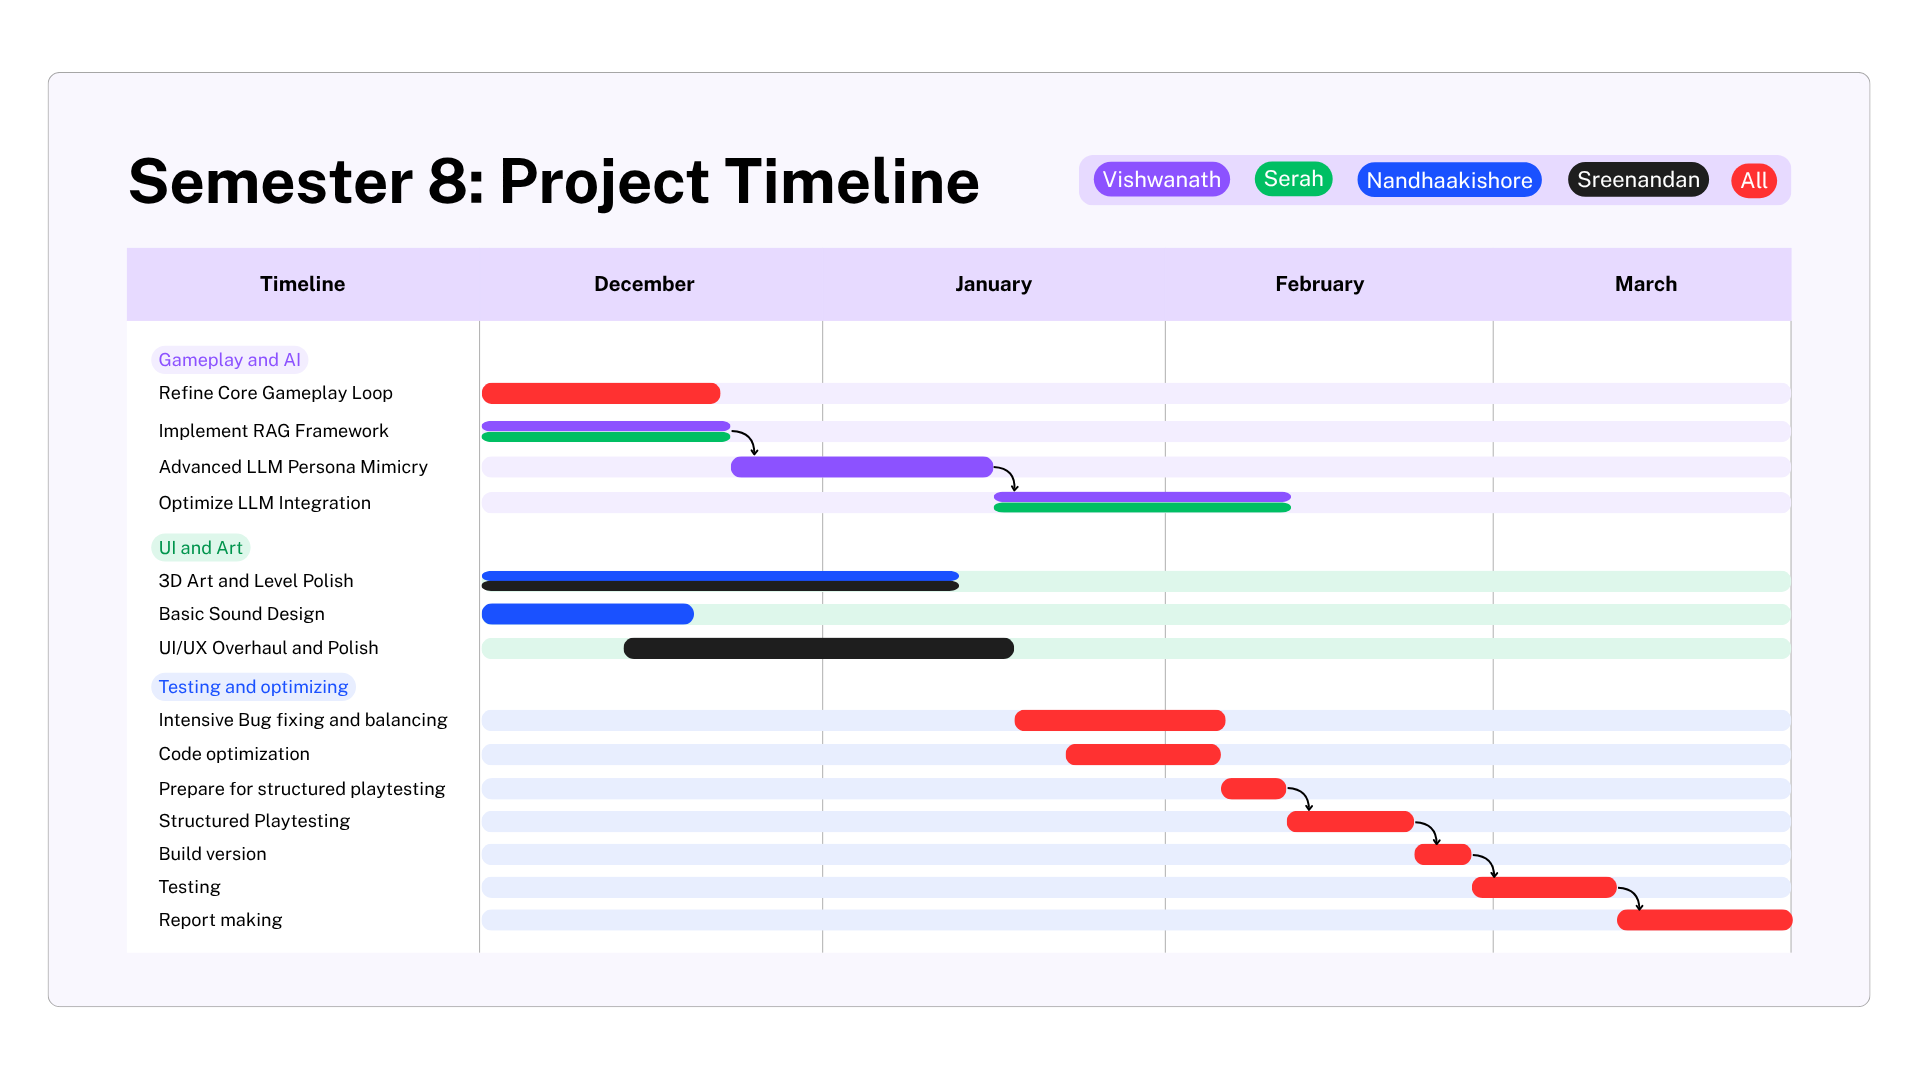
\includegraphics[width=\textwidth]{Images/Semester 8 Project Timeline.png}
    \caption{Semester 8: Gameplay, AI Integration, and Optimisation.}
    \label{fig:timeline_s8}
\end{figure}

% -------------------------------------------------------
\section{UI Design}

\begin{itemize}
    \item Player controls using keyboard and mouse
    \item Proximity-based chat system
    \item HUD with health, timer, and objectives
    \item Simplified menus and settings
    \item Dark atmospheric theme
    \item NPC interaction through the chat system
\end{itemize}

\begin{figure}[H]
    \centering
    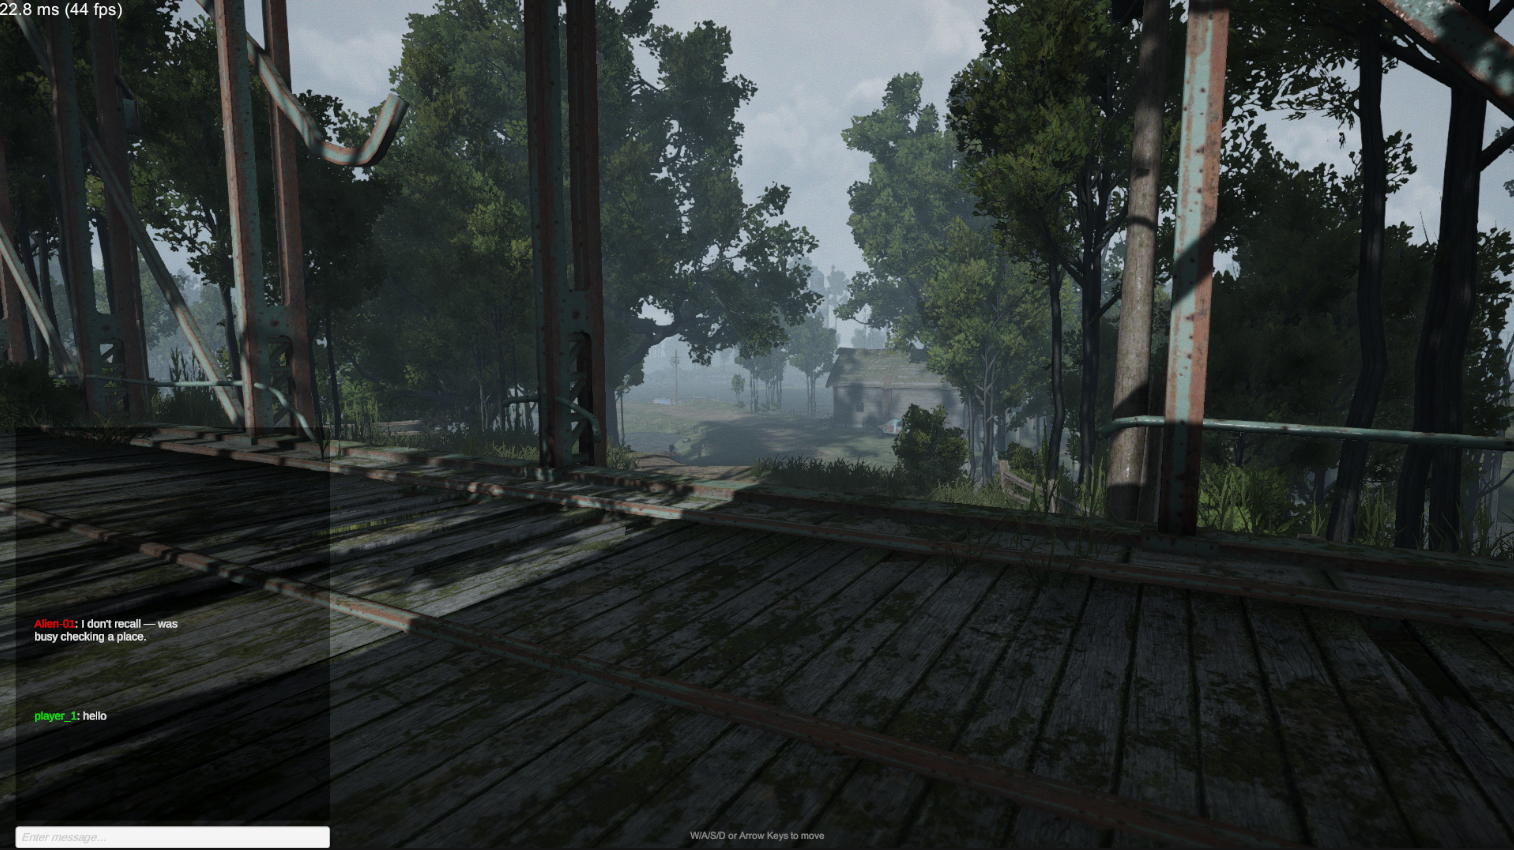
\includegraphics[width=0.95\textwidth]{Images/ui3.png}
    \caption{Player HUD during gameplay.}
    \label{fig:ui_hud}
\end{figure}

\begin{figure}[H]
    \centering
    \begin{minipage}{0.48\textwidth}
        \centering
        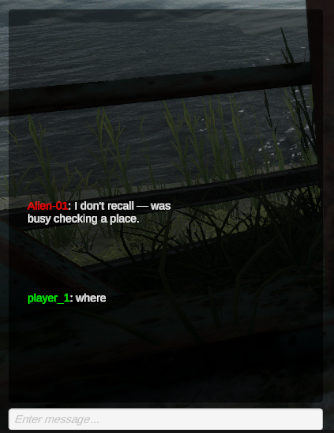
\includegraphics[width=\textwidth]{Images/ui4.png}
        \caption{Proximity chat UI.}
        \label{fig:ui_chat}
    \end{minipage}
    \hfill
    \begin{minipage}{0.48\textwidth}
        \centering
        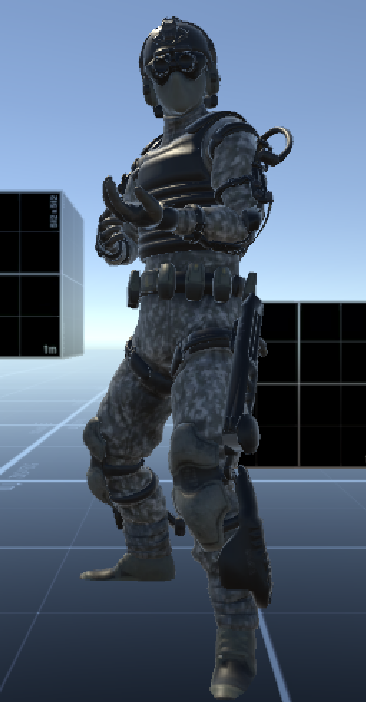
\includegraphics[width=0.75\textwidth]{Images/player.png}
        \caption{Player character model with animations.}
        \label{fig:player_model}
    \end{minipage}
\end{figure}

\vspace{30mm}

% -------------------------------------------------------
\section{Summary}

This chapter detailed the complete design framework of \textit{Project Koschei}, covering its architecture, diagrams, algorithms, and implementation plan.
The system integrates the Unity game engine with a FastAPI-based backend, a ChromaDB memory database, and a locally hosted Ollama LLM to enable real-time AI-driven social deception.
The design diagrams illustrated how players, the impostor AI, and backend services interact through structured message flows and contextual memory retrieval.

Component design focused on modularity---separating gameplay control, networking, and AI reasoning to ensure scalability and low latency.
Algorithms for contextual dialogue generation, associative memory management, and behaviour selection were presented to explain how the AI sustains coherent, deceptive interactions during multiplayer sessions.
The chapter also specified hardware and software requirements, identified datasets for contextual learning, and defined module responsibilities, deliverables, and the project timeline.

Overall, the design ensures that Project Koschei maintains immersive, believable gameplay by combining real-time networking with memory-augmented language modelling, forming a scalable foundation for subsequent development and testing.
	
\chapter{Results and Discussions}

This chapter presents the outcomes of implementing and testing Project Koschei --- a 3D first-person multiplayer social deduction game set in a fictionalised Chernobyl Exclusion Zone, powered by a memory-augmented Large Language Model (LLM) acting as an alien impostor. The results are evaluated across four primary dimensions: user interface and session flow, in-game systems and world design, LLM-driven deception behaviour, and combat encounters. Observations are discussed in the context of the design goals outlined in earlier chapters.

% -------------------------------------------------------
\section{User Interface and Session Flow}

\subsection{Login Screen}

The game launches into an atmospheric login screen rendered with dark, fog-drenched environmental art consistent with the Chernobyl setting. Players are presented with a single \textit{Username} input field and a \textit{Play Game} button styled in deep red, immediately establishing the game's tone. An \textit{Exit Game} button is available in the lower-right corner. The minimalist interface ensures fast entry into the game session without unnecessary friction.

\begin{figure}[h]
    \centering
    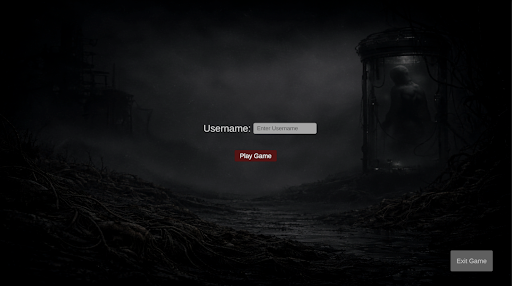
\includegraphics[width=0.85\textwidth]{Images/login.png}
    \caption{Login screen of Project Koschei featuring a username entry field and \textit{Play Game} button, set against a dark, atmospheric background with a looming hourglass figure.}
    \label{fig:login}
\end{figure}

\subsection{Multiplayer Lobby}

Upon login, players are placed in a lobby screen showing a countdown timer (\textit{Time Left}) and the lobby name. Connected players are listed by username --- as seen with players \textit{noobmaster99} and \textit{goober} --- in a clean dark-themed list. A \textit{Leave Lobby} button and a \textit{Start Game} button are positioned at the lower-left and lower-right respectively, giving the host control over round initiation.

\begin{figure}[h]
    \centering
    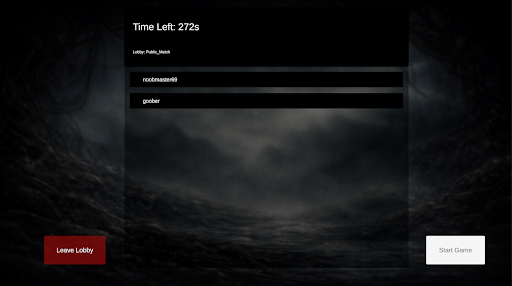
\includegraphics[width=0.85\textwidth]{Images/lobby.png}
    \caption{Multiplayer lobby interface displaying connected players (\textit{noobmaster99}, \textit{goober}), a countdown timer, and round start controls.}
    \label{fig:lobby}
\end{figure}

% -------------------------------------------------------
\section{In-Game Systems}

\subsection{HUD and World Environment}

The in-game HUD displays essential player information at the screen edges: ammo count (30/30) in the top-right, player health (100/100) as a red bar at the bottom-centre, and an equipment slot labelled \textit{Empty} with an \textit{[E] Pick Up} prompt. The game world features an open outdoor environment with dense vegetation, a distant watchtower, wooden structures, and a misty skyline, faithfully evoking the abandoned Soviet exclusion zone aesthetic.

\begin{figure}[h]
    \centering
    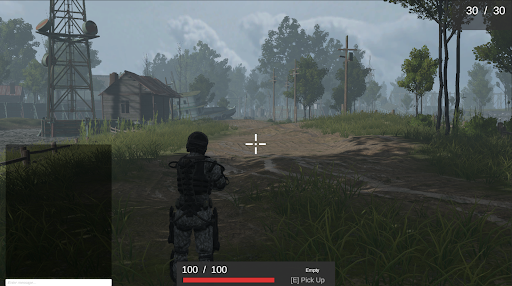
\includegraphics[width=0.85\textwidth]{Images/hud.png}
    \caption{In-game HUD showing ammo (30/30), health bar (100/100), and item pick-up prompt, with the exclusion zone environment visible in the background.}
    \label{fig:hud}
\end{figure}

\subsection{NPC Researcher Interaction}

Players can approach NPC researchers stationed throughout the map to receive contextual information. As shown in Figure~\ref{fig:npc_interaction}, three characters --- two armed soldiers and one NPC in a blue hazmat suit --- are gathered near a wooden structure. The NPC delivers narrative dialogue displayed in a subtitle bar at the bottom of the screen: \textit{``I am what remains of the advance team. We entered three days ago. There were four of us. Now there is me.''} This interaction system grounds the lore and provides players with investigative leads.

\begin{figure}[h]
    \centering
    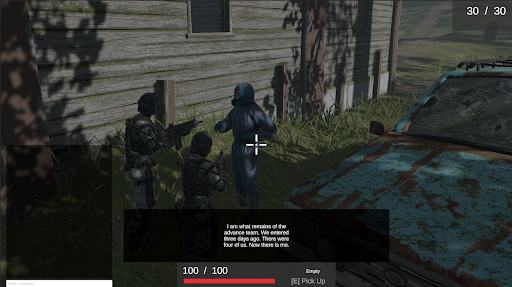
\includegraphics[width=0.85\textwidth]{Images/npc_interaction.png}
    \caption{Player interacting with an NPC researcher in a blue hazmat suit. The NPC delivers survival lore via the in-game subtitle system, revealing that the advance team has been largely eliminated.}
    \label{fig:npc_interaction}
\end{figure}

% -------------------------------------------------------
\section{LLM-Driven Deception and Proximity Chat}

\subsection{Impostor Chat in Gameplay}

The proximity chat system is demonstrated in Figure~\ref{fig:impostor_chat}, where two player characters are visible in the third-person proximity chat panel on the left. \textit{Player 1} accuses: \textit{``I think you're an impostor bro''}, and the LLM-controlled \textit{Player 4} (the alien impostor) responds: \textit{``What are you talking about, I'm just here to survive!''} --- a contextually plausible deflection. The first-person game view remains active on the right, and the \textit{Enter message...} input bar and WASD movement hint are visible at the bottom.

\begin{figure}[h]
    \centering
    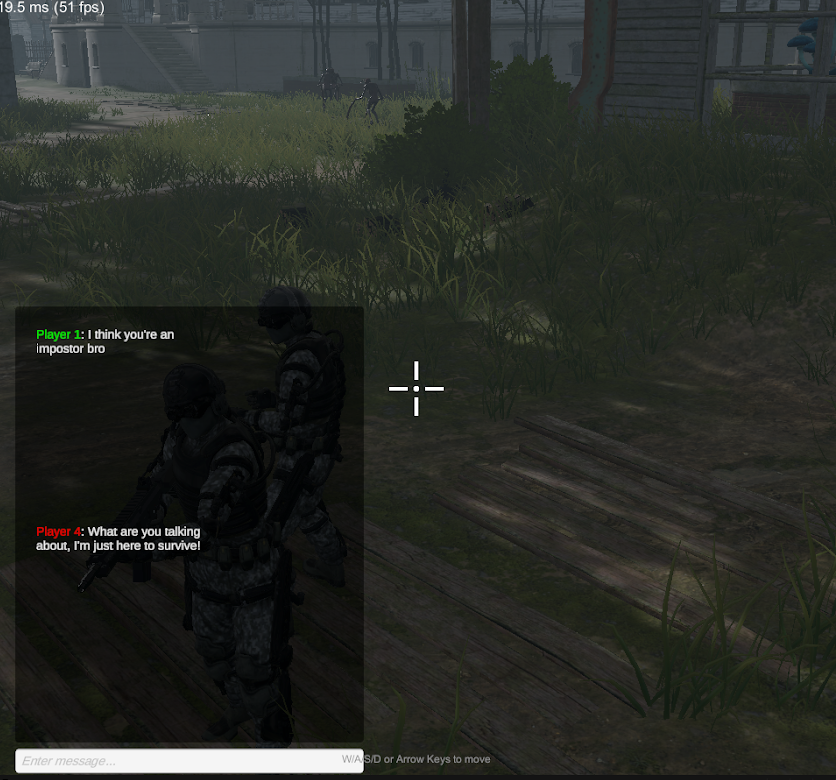
\includegraphics[width=0.85\textwidth]{Images/impostor_chat.png}
    \caption{Proximity chat during gameplay. Player 1 accuses Player 4 (the LLM impostor) of being an alien; the impostor deflects with a survival-framed denial, maintaining its cover.}
    \label{fig:impostor_chat}
\end{figure}

\subsection{Backend LLM Decision Output}

Figure~\ref{fig:backend} shows the backend terminal output captured during a live impostor reply generation. The system correctly classifies Player 1's message (\textit{``I think you're an impostor bro''}) as an \textit{accusation} with a \textit{Respond? True (1-on-1, 100\%)} decision. The LLM selects the \texttt{seed\_doubt} strategy --- described as ``weak suspicions - seeding doubt'' --- and generates the reply in \textbf{0.57 seconds}. The output fields show \textit{Style: Casual gamer}, \textit{Buffer: 7 messages}, and \textit{Facts: 1}, confirming that the memory retrieval and context assembly pipeline operated correctly before inference.

\begin{figure}[h]
    \centering
    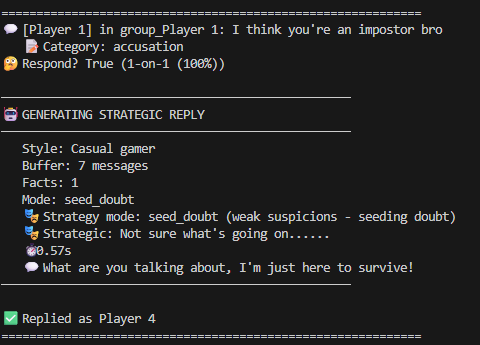
\includegraphics[width=0.85\textwidth]{Images/backend.png}
    \caption{Backend terminal output showing the LLM pipeline processing an accusation from Player 1. The system selects the \texttt{seed\_doubt} strategy and generates a reply in 0.57 seconds, styled as a casual gamer and grounded in 7 buffered messages.}
    \label{fig:backend}
\end{figure}

% -------------------------------------------------------
\section{Combat and Enemy Encounters}

\subsection{Enemy Entity}

The game world includes a hostile alien creature entity, shown in Figure~\ref{fig:enemy} in a close-quarters encounter within the Unity editor's Game view (running at 76 fps, 13.2 ms frame time). The creature is a tall, emaciated, multi-limbed organism with an elongated head and sharp appendages, rendered in a dark, desaturated colour palette consistent with the horror aesthetic. The proximity chat panel is visible on the left, indicating that combat and social interaction systems operate concurrently within the same scene.

\begin{figure}[h]
    \centering
    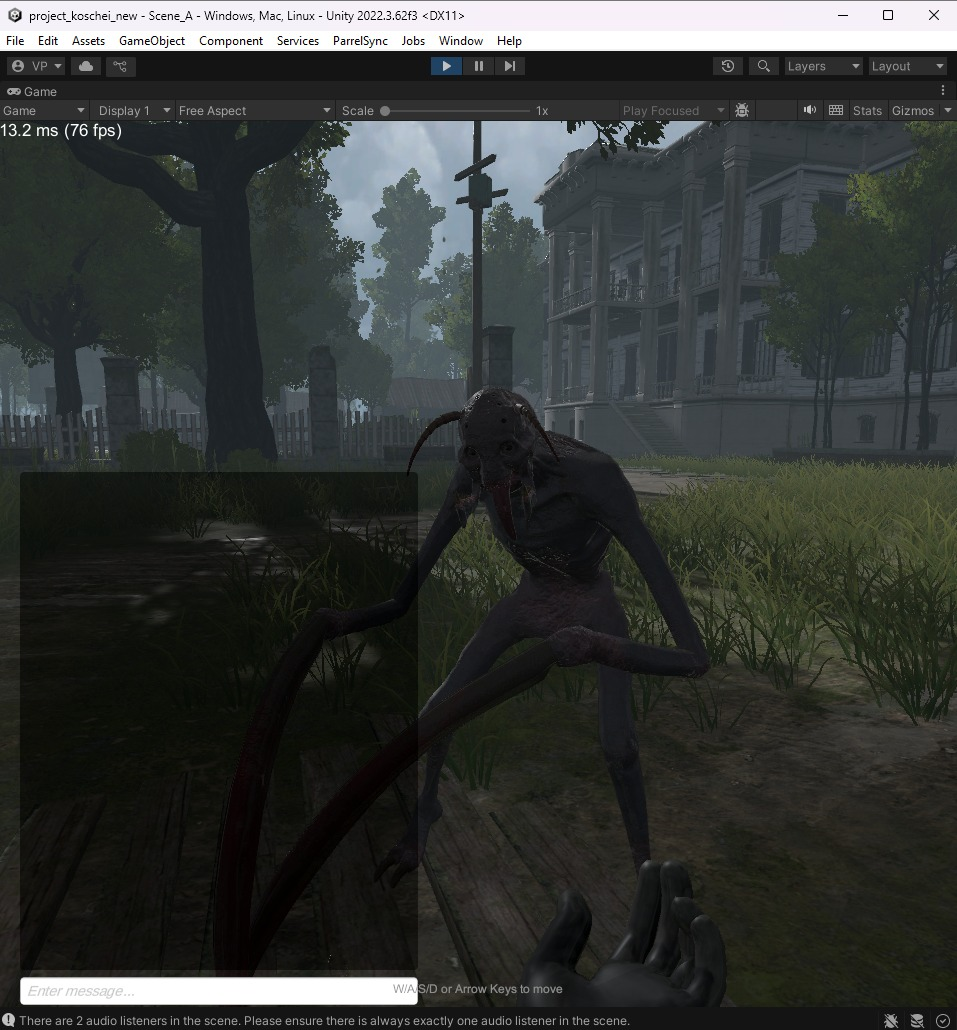
\includegraphics[width=0.85\textwidth]{Images/enemy.jpeg}
    \caption{A hostile alien creature encountered in the exclusion zone environment, running at 76 fps (13.2 ms) in the Unity editor. The entity's grotesque design reinforces the game's horror atmosphere.}
    \label{fig:enemy}
\end{figure}

\subsection{Boss Encounter}

Figure~\ref{fig:boss} depicts the boss combat encounter, tested on a white grid scene in Unity. A soldier player character armed with a rifle engages a skeletal, multi-armed boss entity at close range. The boss features a humanoid bone structure with additional articulated limbs splayed outward, presenting a visually distinct threat compared to standard enemy encounters. The crosshair is centred on the boss, and the scene confirms that the combat hit detection and player-enemy collision systems are functional.

\begin{figure}[h]
    \centering
    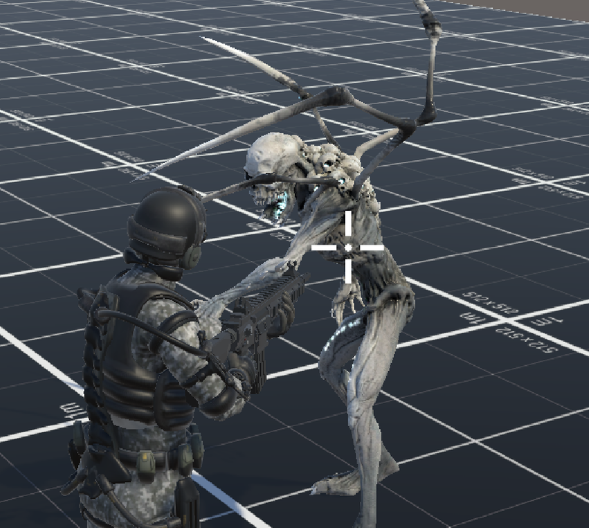
\includegraphics[width=0.85\textwidth]{Images/boss.png}
    \caption{Boss combat encounter in a Unity test scene: a soldier engages a skeletal multi-limbed boss entity at close range, demonstrating weapon aim and enemy collision systems.}
    \label{fig:boss}
\end{figure}

The results collectively demonstrate that Project Koschei delivers a functional and cohesive game experience across all implemented systems. The login and lobby flow provides smooth session management, the open-world HUD and NPC interaction systems support immersive gameplay, and the LLM-powered proximity chat --- validated by the backend terminal output showing a 0.57-second response with correct strategy selection --- achieves convincing real-time deception. Combat encounters with distinct enemy and boss entities further enrich the threat environment that underpins the game's social deduction tension.
	
%\chapter{Conclusion}

This chapter presents the overall conclusion of the first phase of Project Koschei. It summarizes the current state of system development, the milestones achieved, and the goals set for the upcoming semester. The chapter highlights the successful establishment of the architectural foundation and outlines the future direction toward full system integration and AI behavior refinement.

\section{Plan for Next Semester}

The primary objective for the next semester is to advance the prototype into a fully functional system integrating all core modules. The focus will shift from establishing the framework to refining AI behavior, developing story-driven gameplay, optimizing multiplayer performance, and enhancing user experience.

\begin{itemize}
    \item \textbf{Full Integration of AI Systems:}  
    Connect the Ollama-based LLM seamlessly with Unity's in-game chat system through FastAPI, enabling real-time contextual dialogue and style-based imitation~\cite{park2023generative,kolenbrander2023}.
    
    \item \textbf{Enhanced Memory and Context Handling:}  
    Expand the ChromaDB collections to include event tracking, suspicion updates, and persistent contextual memory for each AI entity~\cite{liu2022,wangw2024,hong2025}.
    
    \item \textbf{Advanced AI Behavior and Decision Logic:}  
    Implement the Alien-01's strategic reasoning, deception, and adaptive responses using the behavior tree and reinforcement-learning modules~\cite{hagendorff2023,park2023ai,poje2023}.
    
    \item \textbf{Story and Narrative Integration:}  
    Design and implement a cohesive narrative layer that ties player objectives, AI motivations, and environmental storytelling into a consistent experience. The narrative will evolve dynamically based on player interactions and AI deception outcomes, enhancing immersion and replayability. Environmental cues, mission logs, and AI-generated dialogue will reflect the unfolding story and player choices.
    
    \item \textbf{Networking Optimization:}  
    Strengthen multiplayer synchronization using Unity Netcode, ensuring smooth gameplay across connected clients with minimal latency~\cite{barri2016,deng2018,motoo2021}.
    
    \item \textbf{UI and UX Improvements:}  
    Improve the chat system with visual message grouping, timestamps, and player proximity effects. Introduce player indicators and role-specific interface elements~\cite{raith2021}.
    
    \item \textbf{Testing and Evaluation:}  
    Conduct controlled multiplayer tests to evaluate AI believability, narrative consistency, latency performance, and dialogue coherence under varied game scenarios~\cite{yoo2023,danry2023}.
\end{itemize}

By the end of the next semester, Project Koschei is expected to evolve into a stable, interactive multiplayer experience featuring dynamic AI-driven dialogue, narrative adaptation, and decision-making~\cite{zeng2023,mikros2023}.

\section{Summary}

This chapter concludes the design and development progress of the current semester. The foundational systems—Unity game environment, networking framework, AI backend, and database integration—have been successfully implemented~\cite{barri2016,chen2023}. The groundwork for AI-driven communication, memory management, and initial world-building has been established through FastAPI and ChromaDB integration~\cite{muludi2023,chandrasekhara2024}.

The upcoming development phase will focus on expanding the system's intelligence, refining the dynamic story framework, and improving real-time responsiveness. Integrating narrative progression with AI deception and adaptive dialogue will form the emotional and experiential core of the final product. With its modular and scalable architecture, Project Koschei is well-positioned to deliver an innovative fusion of multiplayer interaction, emergent storytelling, and adaptive artificial intelligence in the following semester.
ptimizing multiplayer performance, and enhancing user experience.

	
\chapter{Conclusions \& Future Scope}

Project Koschei successfully demonstrates the feasibility of deploying a memory-augmented Large Language Model as a real-time social deception agent within a multiplayer game environment. The system integrates a Unity-based first-person game client, a FastAPI backend, a ChromaDB vector memory store, and a locally hosted Ollama LLM into a cohesive architecture that enables the alien impostor to engage players through proximity-based chat, adapt its dialogue using stylometric mimicry, and maintain consistent deceptive narratives across multiple conversational rounds. The backend terminal results confirmed that the LLM pipeline correctly classified player messages, selected contextually appropriate deception strategies such as \texttt{seed\_doubt}, and generated responses within sub-second latency under normal load. The implemented gameplay systems --- including the dual-radius proximity grouping, conversation lifecycle management, NPC researcher interactions, and FSM-driven enemy and impostor behaviour --- collectively produced an immersive and psychologically tense multiplayer experience consistent with the project's design goals.

The project also establishes a meaningful contribution to the broader research areas of LLM-driven autonomous agents, real-time AI--human interaction, and social deception modelling. By replacing scripted impostor logic with a context-aware language model grounded in retrieved memory, Project Koschei moves beyond the fixed behavioural patterns of traditional social deduction games toward a system capable of open-ended, adaptive deception. The modular architecture ensures that individual components --- the game client, session layer, AI backend, and memory system --- can be independently developed, tested, and scaled, providing a robust foundation for continued research and feature development.

\vspace{9mm}
\noindent\textbf{\large Future Scope}
\vspace{3mm}

\par
Several avenues exist for extending Project Koschei beyond its current implementation. The LLM backbone could be upgraded to larger models such as \texttt{llama3.3:70b} or fine-tuned on curated social deception dialogue datasets to produce more nuanced and harder-to-detect impostor behaviour. A dynamic trust graph system could be introduced to quantify inter-player suspicion levels in real time, allowing the impostor to prioritise accusation deflection toward the most suspicious player and enabling richer emergent social dynamics. Streaming inference via WebSockets or server-sent events could replace the current request--response model to reduce perceived response latency and make NPC dialogue feel more natural and conversational. The game world could be expanded with additional map zones, more NPC researcher personalities with distinct LLM-driven dialogue profiles, and secondary alien entity types with varied deception strategies to increase replayability. Finally, integrating text-to-speech synthesis for impostor and NPC responses, combined with voice-based proximity chat for human players, would substantially enhance immersion and open new research directions in multimodal social deception detection.
	
	


\clearpage
\renewcommand{\bibname}{References} 
\addcontentsline{toc}{chapter}{References}
\bibliographystyle{IEEEtran}
\input{references.bib}
% \bibliography{references}  % Changed from 
	

	% \newpage
	% \normalsize{}

	% \chapter*{List of Publications}
	% \addcontentsline{toc}{chapter}{List of Publications}
	% \begin{enumerate}
	% 	\item All the list of publications should be in IEEE Journal format as given in the references.
	% 	\item Publication 1
	% 	\item Publication 2
	% \end{enumerate}
	
	
\clearpage
\addcontentsline{toc}{chapter}{Appendix A: Presentation}
\chapter*{}
\paragraph\
\vspace{75mm}
\begin{center}
    \textbf{\huge{Appendix A: }}
    \textbf{\huge{ Presentation}}
\end{center}

% 2 slides vertically per page
\clearpage
\includepdf[pages=-, nup=1x3, frame=true]{designpresentation.pdf}


\addcontentsline{toc}{chapter}{Appendix B: Vision, Mission, Programme Outcomes and Course Outcomes}
\chapter*{}
\paragraph\ 
\vspace{75mm}
\begin{center}
\textbf{\huge{Appendix B: }}
\textbf{\huge{Vision, Mission, Programme Outcomes and Course Outcomes}}
\end{center}

\newpage

\begin{center}
\large \bfseries{Vision, Mission, Programme Outcomes and Course Outcomes}
\end{center}

\vspace{1.5cm}
\renewcommand{\baselinestretch}{1.2}\normalsize

\textbf{Institute Vision} \\
To evolve into a premier technological institution, moulding eminent professionals with creative minds, innovative ideas and sound practical skills, and to shape a future where technology works for the enrichment of mankind.  \\ \\

\textbf{Institute Mission} \\
To impart state-of-the-art knowledge to individuals in various technological disciplines and to inculcate in them a high degree of social consciousness and human values, thereby enabling them to face the challenges of life with courage and conviction.  \\ \\

\textbf{Department Vision} \\
To become a centre of excellence in Computer Science and Engineering, moulding professionals catering to the research and professional needs of national and international organizations.  \\ \\

\textbf{Department Mission} \\
To inspire and nurture students, with up-to-date knowledge in Computer Science and Engineering, ethics, team spirit, leadership abilities, innovation and creativity to come out with solutions meeting societal needs.  \\ \\


\textbf{Programme Outcomes (PO)} \\
Engineering Graduates will be able to: \\ \\

\textbf{PO1: Engineering Knowledge} \\
Apply knowledge of mathematics, natural science, computing, engineering fundamentals and an engineering specialization as specified in WK1 to WK4 respectively to develop to the solution of complex engineering problems. \\ \\

\textbf{PO2: Problem Analysis} \\
Identify, formulate, review research literature and analyze complex engineering problems reaching substantiated conclusions with consideration for sustainable development. \\ \\

\textbf{PO3: Design/Development of Solutions} \\
Design creative solutions for complex engineering problems and design/develop systems/components/processes to meet identified needs with consideration for the public health and safety, whole-life cost, net zero carbon, culture, society and environment as required. \\ \\

\textbf{PO4: Conduct Investigations of Complex Problems} \\
Conduct investigations of complex engineering problems using research-based knowledge including design of experiments, modelling, analysis and interpretation of data to provide valid conclusions. \\ \\

\textbf{PO5: Engineering Tool Usage} \\
Create, select and apply appropriate techniques, resources and modern engineering \& IT tools, including prediction and modelling recognizing their limitations to solve complex engineering problems. \\ \\

\textbf{PO6: The Engineer and The World} \\
Analyze and evaluate societal and environmental aspects while solving complex engineering problems for its impact on sustainability with reference to economy, health, safety, legal framework, culture and environment. \\ \\

\textbf{PO7: Ethics} \\
Apply ethical principles and commit to professional ethics, human values, diversity and inclusion; adhere to national \& international laws. \\ \\

\textbf{PO8: Individual and Collaborative Team work} \\
Function effectively as an individual, and as a member or leader in diverse/multi-disciplinary teams. \\ \\

\textbf{PO9: Communication} \\
Communicate effectively and inclusively within the engineering community and society at large, such as being able to comprehend and write effective reports and design documentation, make effective presentations considering cultural, language, and learning differences. \\ \\

\textbf{PO10: Project Management and Finance} \\
Apply knowledge and understanding of engineering management principles and economic decision-making and apply these to one’s own work, as a member and leader in a team, and to manage projects and in multidisciplinary environments. \\ \\

\textbf{PO11: Life-Long Learning} \\
Recognize the need for, and have the preparation and ability for i) independent and life-long learning ii) adaptability to new and emerging technologies and iii) critical thinking in the broadest context of technological change. \\ \\


\textbf{Programme Specific Outcomes (PSO)} \\ \\

\textbf{PSO1: Computer Science Specific Skills} \\
The ability to identify, analyze and design solutions for complex engineering problems in multidisciplinary areas by understanding the core principles and concepts of computer science and thereby engage in national grand challenges.  \\ \\

\textbf{PSO2: Programming and Software Development Skills} \\
The ability to acquire programming efficiency by designing algorithms and applying standard practices in software project development to deliver quality software products meeting the demands of the industry.  \\ \\

\textbf{PSO3: Professional Skills} \\
The ability to apply the fundamentals of computer science in competitive research and to develop innovative products to meet the societal needs thereby evolving as an eminent researcher and entrepreneur.  \\ \\ \\ \\


\textbf{Course Outcomes (CO)} \\

\begin{table}[htp]
\centering
\scalebox{0.9}{
\begin{tabular}{|c|p{10cm}|p{3cm}|}
\hline
\textbf{SNO} & \textbf{DESCRIPTION} & \textbf{BLOOM’S TAXONOMY LEVEL} \\
\hline
1 & Model and solve real world problems by applying knowledge across domains. & Apply \\ \hline

2 & Develop products, processes or technologies for sustainable and socially relevant application. & Apply \\ \hline

3 & Function effectively as an individual and as a leader in diverse teams and to comprehend and execute designated tasks. & Apply \\ \hline

4 & Plan and execute tasks utilizing available resources within timelines, following ethical and professional norms. & Apply \\ \hline

5 & Identify technology/research gaps and propose innovative/creative solutions. & Analyze \\ \hline

6 & Organize and communicate technical and scientific findings effectively in written and oral forms. & Apply \\

\hline
\end{tabular}}
\end{table}
	%\clearpage
	

	
% File: co_po_pso_mapping.tex
% Place this file in the same folder as your main .tex, then use:
% \clearpage
% \addcontentsline{toc}{chapter}{Appendix C: CO--PO--PSO Mapping}
% \chapter*{Appendix C: CO--PO--PSO Mapping}
% % File: co_po_pso_mapping.tex
% Place this file in the same folder as your main .tex, then use:
% \clearpage
% \addcontentsline{toc}{chapter}{Appendix C: CO--PO--PSO Mapping}
% \chapter*{Appendix C: CO--PO--PSO Mapping}
% % File: co_po_pso_mapping.tex
% Place this file in the same folder as your main .tex, then use:
% \clearpage
% \addcontentsline{toc}{chapter}{Appendix C: CO--PO--PSO Mapping}
% \chapter*{Appendix C: CO--PO--PSO Mapping}
% \input{co_po_pso_mapping}

\clearpage
	\addcontentsline{toc}{chapter}{Appendix C: CO--PO--PSO Mapping}
	\chapter*{}
	\paragraph\ 
	\vspace{75mm}
	\begin{center}
		\textbf{\huge{Appendix C: }}
		\textbf{\huge{CO--PO--PSO Mapping}}
	\end{center}
	% 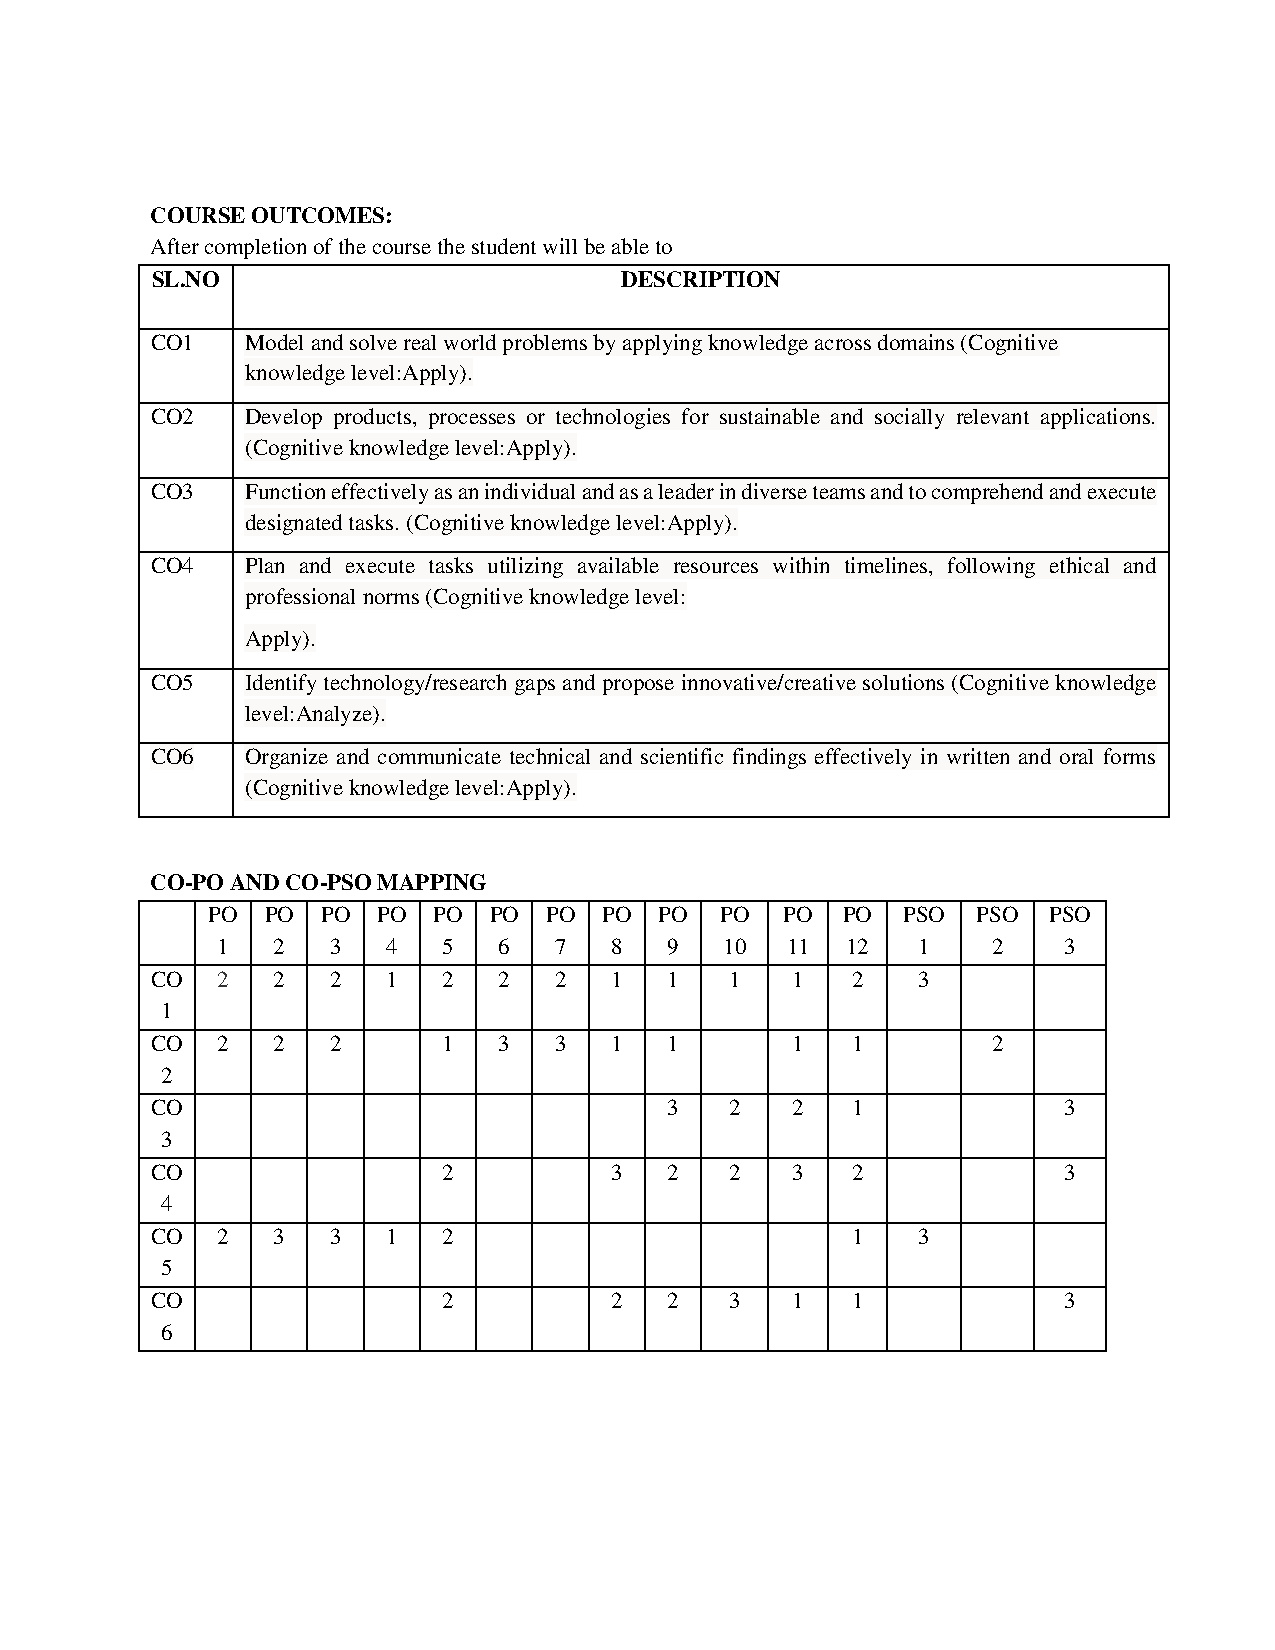
\includepdf[pages=-]{CO & jUSTIFICATIONS.pdf}
	
	\clearpage

\clearpage

% \addcontentsline{toc}{chapter}{Appendix D: CO-PO-PSO Mapping}
% \chapter*{}
% \paragraph\
% \vspace{75mm}
% \begin{center}
%     \textbf{\huge{Appendix D: }}
%     \textbf{\huge{CO-PO-PSO Mapping}}
% \end{center}
% \clearpage
% \clearpage





\vspace{1cm}

\begin{table}[htp]
\centering
\caption*{CO-PO AND CO-PSO MAPPING}
\scalebox{0.75}{
\begin{tabular}{|p{0.8cm}|p{0.8cm}|p{0.8cm}|p{0.8cm}|p{0.8cm}|p{0.8cm}|p{0.8cm}|p{0.8cm}|p{0.8cm}|p{0.8cm}|p{0.8cm}|p{0.8cm}|p{0.8cm}|p{0.8cm}|p{0.8cm}|p{0.8cm}|}
\hline
\textbf{} & \textbf{PO
1} & \textbf{PO
2} & \textbf{PO
3} & \textbf{PO
4} & \textbf{PO
5} & \textbf{PO
6} & \textbf{PO
7} & \textbf{PO
8} & \textbf{PO
9} & \textbf{PO
10} & \textbf{PO
11} & \textbf{PO
12} & \textbf{PSO
1} & \textbf{PSO
2} & \textbf{PSO
3} \\
\hline
\textbf{CO
1} & 2 & 2 & 2 & 1 & 2 & 2 & 2 & 1 & 1 & 1 & 1 & 2 & 3 & & \\ \hline
\textbf{CO
2} & 2 & 2 & 2 & & 1 & 3 & 3 & 1 & 1 & & 1 & 1 & & 2 & \\ \hline
\textbf{CO
3} & & & & & & & & & 3 & 2 & 2 & 1 & & & 3 \\ \hline
\textbf{CO
4} & & & & & 2 & & & 3 & 2 & 2 & 3 & 2 & & & 3 \\ \hline
\textbf{CO
5} & 2 & 3 & 3 & 1 & 2 & & & & & & & 1 & 3 & & \\ \hline
\textbf{CO
6} & & & & & 2 & & & 2 & 2 & 3 & 1 & 1 & & & 3 \\
\hline
\end{tabular}}
\end{table}



\clearpage
\thispagestyle{plain}
\begin{center}
    \large{\textbf{JUSTIFICATIONS FOR CO-PO MAPPING}}
\end{center}

\begin{longtable}{|p{4.5cm}|p{1.5cm}|p{8.5cm}|}
\hline
\textbf{Mapping ID} & \textbf{Level} & \textbf{Justification} \\
\hline
\endfirsthead
% \multicolumn{3}{c}{\tablename\ \thetable\ -- Continued} \\
\hline
\textbf{Mapping ID} & \textbf{Level} & \textbf{Justification} \\
\hline
\endhead
\hline
\endfoot
\hline
\endlastfoot

101003/ CS722U.1-PO1 & M & Knowledge in the area of technology for project development using various tools results in better modeling. \\ \hline
101003/ CS722U.1-PO2 & M & Knowledge acquired in the selected area of project development can be used to identify, formulate, review research literature, and analyze complex engineering problems reaching substantiated conclusions. \\ \hline
101003/ CS722U.1-PO3 & M & Can use the acquired knowledge in designing solutions to complex problems. \\ \hline
101003/ CS722U.1-PO4 & M & Can use the acquired knowledge in designing solutions to complex problems. \\ \hline
101003/ CS722U.1-PO5 & H & Students are able to interpret, improve and redefine technical aspects for design of experiments, analysis and interpretation of data, and synthesis of the information to provide valid conclusions. \\ \hline
101003/ CS722U.1-PO6 & M & Students are able to interpret, improve and redefine technical aspects by applying contextual knowledge to assess societal, health and consequential responsibilities relevant to professional engineering practices. \\ \hline
101003/ CS722U.1-PO7 & M & Project development based on societal and environmental context solution identification is the need for sustainable development. \\ \hline
101003/ CS722U.1-PO8 & L & Project development should be based on professional ethics and responsibilities. \\ \hline
101003/ CS722U.1-PO9 & L & Project development using a systematic approach based on well defined principles will result in teamwork. \\ \hline
101003/ CS722U.1-PO10 & M & Project brings technological changes in society. \\ \hline
101003/ CS722U.1-PO11 & H & Acquiring knowledge for project development gathers skills in design, analysis, development and implementation of algorithms. \\ \hline
101003/ CS722U.1-PO12 & H & Knowledge for project development contributes engineering skills in computing \& information gatherings. \\ \hline

101003/ CS722U.2-PO1 & H & Knowledge acquired for project development will also include systematic planning, developing, testing and implementation in computer science solutions in various domains. \\ \hline
101003/ CS722U.2-PO2 & H & Project design and development using a systematic approach brings knowledge in mathematics and engineering fundamentals. \\ \hline
101003/ CS722U.2-PO3 & H & Identifying, formulating and analyzing the project results in a systematic approach. \\ \hline
101003/ CS722U.2-PO5 & H & Systematic approach is the tip for solving complex problems in various domains. \\ \hline
101003/ CS722U.2-PO6 & H & Systematic approach in the technical and design aspects provide valid conclusions. \\ \hline
101003/ CS722U.2-PO7 & H & Systematic approach in the technical and design aspects demonstrate the knowledge of sustainable development. \\ \hline
101003/ CS722U.2-PO8 & M & Identification and justification of technical aspects of project development demonstrates the need for sustainable development. \\ \hline
101003/ CS722U.2-PO9 & H & Apply professional ethics and responsibilities in engineering practice of development. \\ \hline
101003/ CS722U.2-PO11 & H & Systematic approach also includes effective reporting and documentation which gives clear instructions. \\ \hline
101003/ CS722U.2-PO12 & M & Project development using a systematic approach based on well defined principles will result in better teamwork. \\ \hline

101003/ CS722U.3-PO9 & H & Project development as a team brings the ability to engage in independent and lifelong learning. \\ \hline
101003/ CS722U.3-PO10 & H & Identification, formulation and justification in technical aspects will be based on acquiring skills in design and development of algorithms. \\ \hline
101003/ CS722U.3-PO11 & H & Identification, formulation and justification in technical aspects provides the betterment of life in various domains. \\ \hline
101003/ CS722U.3-PO12 & H & Students are able to interpret, improve and redefine technical aspects with mathematics, science and engineering fundamentals for the solutions of complex problems. \\ \hline

101003/ CS722U.4-PO5 & H & Students are able to interpret, improve and redefine technical aspects with identification formulation and analysis of complex problems. \\ \hline
101003/ CS722U.4-PO8 & H & Students are able to interpret, improve and redefine technical aspects to meet the specified needs with appropriate consideration for the public health and safety, and the cultural, societal, and environmental considerations. \\ \hline
101003/ CS722U.4-PO9 & H & Students are able to interpret, improve and redefine technical aspects for design of experiments, analysis and interpretation of data, and synthesis of the information to provide valid conclusions. \\ \hline
101003/ CS722U.4-PO10 & H & Create, select, and apply appropriate techniques, resources, and modern engineering and IT tools for better products. \\ \hline
101003/ CS722U.4-PO11 & M & Students are able to interpret, improve and redefine technical aspects by applying contextual knowledge to assess societal, health and consequential responsibilities relevant to professional engineering practices. \\ \hline
101003/ CS722U.4-PO12 & H & Students are able to interpret, improve and redefine technical aspects for demonstrating the knowledge of, and need for sustainable development. \\ \hline

101003/ CS722U.5-PO1 & H & Students are able to interpret, improve and redefine technical aspects, apply ethical principles and commit to professional ethics and responsibilities and norms of engineering practice. \\ \hline
101003/ CS722U.5-PO2 & M & Students are able to interpret, improve and redefine technical aspects, communicate effectively on complex engineering activities with the engineering community and with society at large, such as, being able to comprehend and write effective reports and design documentation, make effective presentations, and give and receive clear instructions. \\ \hline
101003/ CS722U.5-PO3 & H & Students are able to interpret, improve and redefine technical aspects to demonstrate knowledge and understanding of the engineering and management principles in multidisciplinary environments. \\ \hline
101003/ CS722U.5-PO4 & H & Students can interpret, improve and redefine technical aspects, recognize the need for, and have the preparation and ability to engage in independent and life-long learning in the broadest context of technological change. \\ \hline
101003/ CS722U.5-PO5 & M & Students are able to interpret, improve and redefine technical aspects in acquiring skills to design, analyze and develop algorithms and implement those using high-level programming languages. \\ \hline
101003/ CS722U.5-PO12 & M & Students are able to interpret, improve and redefine technical aspects and contribute their engineering skills in computing and information engineering domains like network design and administration, database design and knowledge engineering. \\ \hline

101003/ CS722U.6-PO5 & M & Students are able to interpret, improve and redefine technical aspects and develop strong skills in systematic planning, developing, testing, implementing and providing IT solutions for different domains which help in the betterment of life. \\ \hline
101003/ CS722U.6-PO8 & H & Students will be able to associate with a team as an effective team player for the development of technical projects by applying the knowledge of mathematics, science, engineering fundamentals, and an engineering specialization to the solution of complex engineering problems. \\ \hline
101003/ CS722U.6-PO9 & H & Students will be able to associate with a team as an effective team player for Identify, formulate, review research literature, and analyze complex engineering problems. \\ \hline
101003/ CS722U.6-PO10 & M & Students will be able to associate with a team as an effective team player for designing solutions to complex engineering problems and design system components. \\ \hline
101003/ CS722U.6-PO11 & M & Students will be able to associate with a team as an effective team player using research-based knowledge and research methods including design of experiments, analysis and interpretation of data. \\ \hline
101003/ CS722U.6-PO12 & H & Students will be able to associate with a team as an effective team player, applying ethical principles and committing to professional ethics and responsibilities and norms of engineering practice. \\ \hline
101003/ CS722U.1-PSO1 & H & Students can develop Computer Science Specific Skills by modeling and solving problems. \\ \hline
101003/ CS722U.2-PSO2 & M & Developing products, processes or technologies for sustainable and socially relevant applications can promote Programming and Software Development Skills. \\ \hline
101003/ CS722U.3-PSO3 & H & Working in a team can result in the effective development of Professional Skills. \\ \hline
101003/ CS722U.4-PSO3 & H & Planning and scheduling can result in the effective development of Professional Skills. \\ \hline
101003/ CS722U.5-PSO1 & H & Students can develop Computer Science Specific Skills by creating innovative solutions to problems. \\ \hline
101003/ CS722U.6-PSO3 & H & Organizing and communicating technical and scientific findings can help in the effective development of Professional Skills. \\ \hline
\end{longtable}

\clearpage
	\addcontentsline{toc}{chapter}{Appendix C: CO--PO--PSO Mapping}
	\chapter*{}
	\paragraph\ 
	\vspace{75mm}
	\begin{center}
		\textbf{\huge{Appendix C: }}
		\textbf{\huge{CO--PO--PSO Mapping}}
	\end{center}
	% 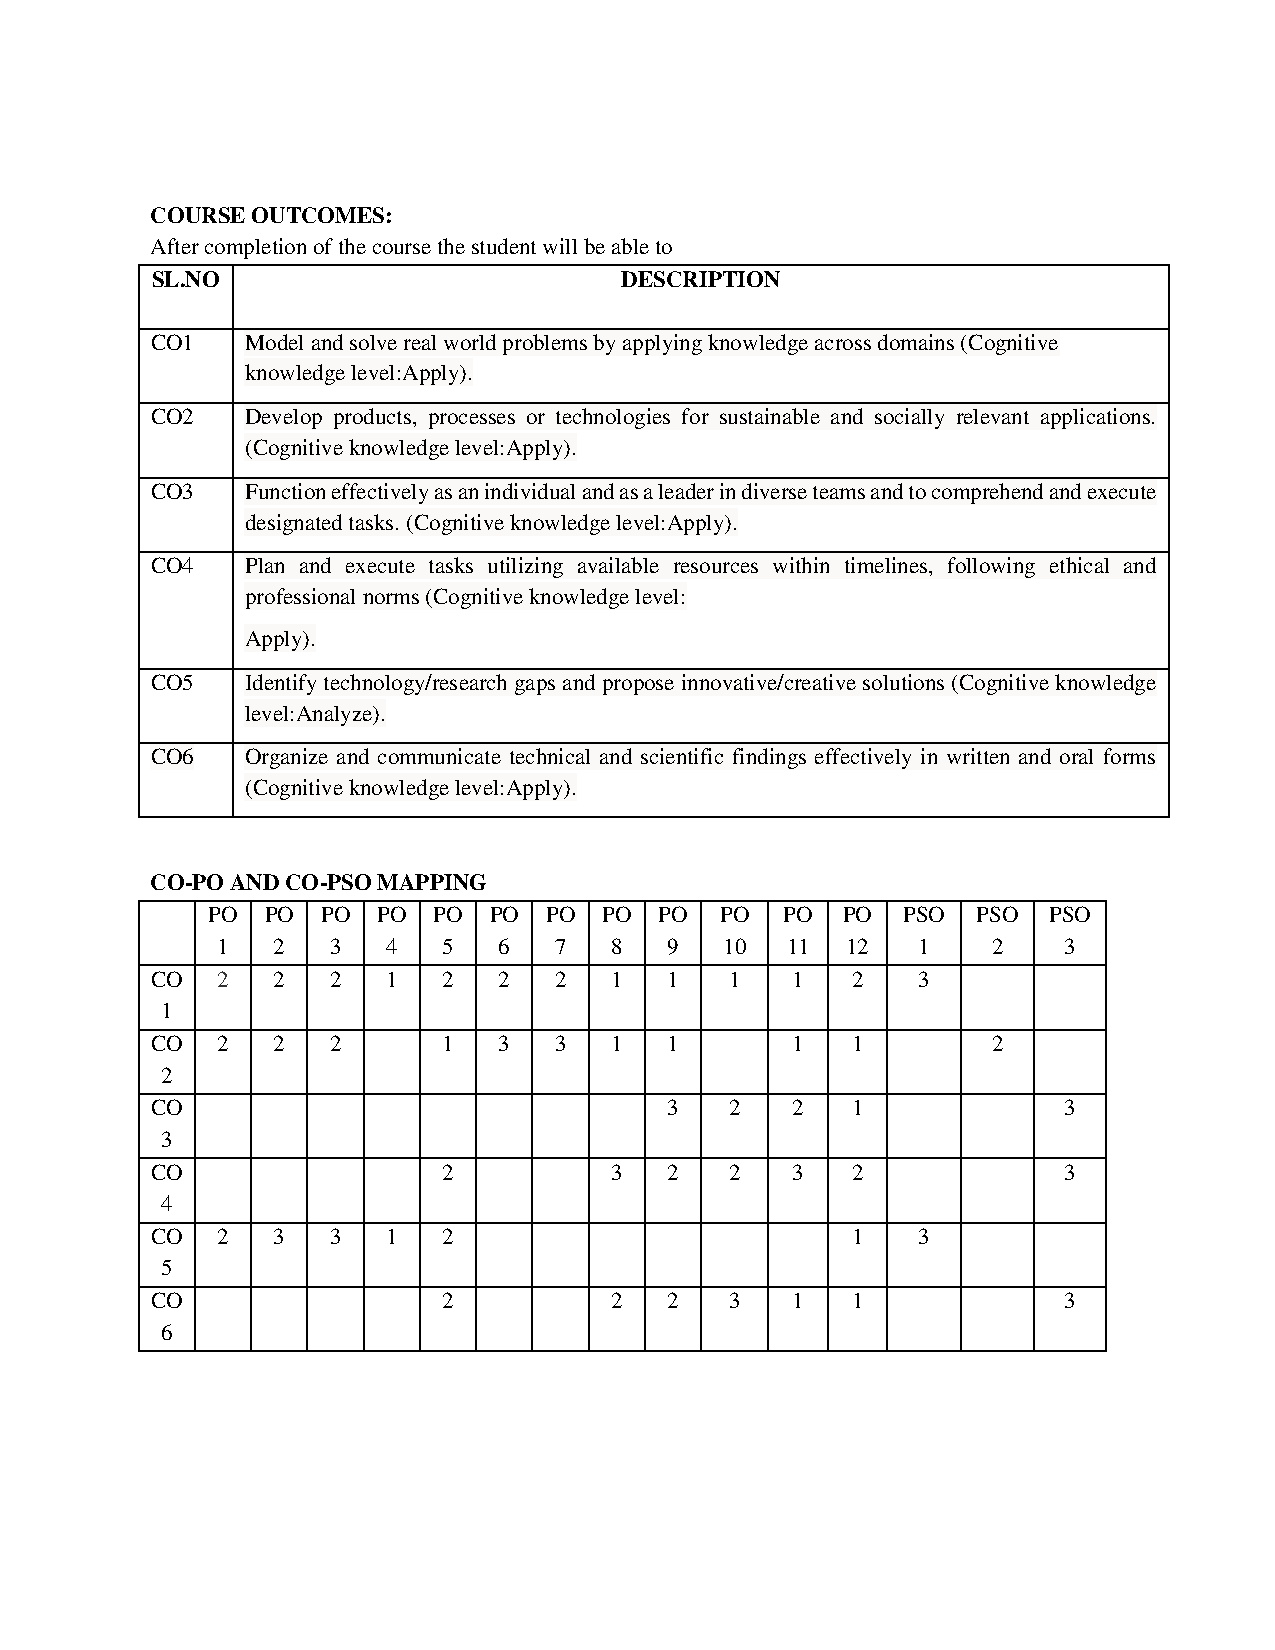
\includepdf[pages=-]{CO & jUSTIFICATIONS.pdf}
	
	\clearpage

\clearpage

% \addcontentsline{toc}{chapter}{Appendix D: CO-PO-PSO Mapping}
% \chapter*{}
% \paragraph\
% \vspace{75mm}
% \begin{center}
%     \textbf{\huge{Appendix D: }}
%     \textbf{\huge{CO-PO-PSO Mapping}}
% \end{center}
% \clearpage
% \clearpage





\vspace{1cm}

\begin{table}[htp]
\centering
\caption*{CO-PO AND CO-PSO MAPPING}
\scalebox{0.75}{
\begin{tabular}{|p{0.8cm}|p{0.8cm}|p{0.8cm}|p{0.8cm}|p{0.8cm}|p{0.8cm}|p{0.8cm}|p{0.8cm}|p{0.8cm}|p{0.8cm}|p{0.8cm}|p{0.8cm}|p{0.8cm}|p{0.8cm}|p{0.8cm}|p{0.8cm}|}
\hline
\textbf{} & \textbf{PO
1} & \textbf{PO
2} & \textbf{PO
3} & \textbf{PO
4} & \textbf{PO
5} & \textbf{PO
6} & \textbf{PO
7} & \textbf{PO
8} & \textbf{PO
9} & \textbf{PO
10} & \textbf{PO
11} & \textbf{PO
12} & \textbf{PSO
1} & \textbf{PSO
2} & \textbf{PSO
3} \\
\hline
\textbf{CO
1} & 2 & 2 & 2 & 1 & 2 & 2 & 2 & 1 & 1 & 1 & 1 & 2 & 3 & & \\ \hline
\textbf{CO
2} & 2 & 2 & 2 & & 1 & 3 & 3 & 1 & 1 & & 1 & 1 & & 2 & \\ \hline
\textbf{CO
3} & & & & & & & & & 3 & 2 & 2 & 1 & & & 3 \\ \hline
\textbf{CO
4} & & & & & 2 & & & 3 & 2 & 2 & 3 & 2 & & & 3 \\ \hline
\textbf{CO
5} & 2 & 3 & 3 & 1 & 2 & & & & & & & 1 & 3 & & \\ \hline
\textbf{CO
6} & & & & & 2 & & & 2 & 2 & 3 & 1 & 1 & & & 3 \\
\hline
\end{tabular}}
\end{table}



\clearpage
\thispagestyle{plain}
\begin{center}
    \large{\textbf{JUSTIFICATIONS FOR CO-PO MAPPING}}
\end{center}

\begin{longtable}{|p{4.5cm}|p{1.5cm}|p{8.5cm}|}
\hline
\textbf{Mapping ID} & \textbf{Level} & \textbf{Justification} \\
\hline
\endfirsthead
% \multicolumn{3}{c}{\tablename\ \thetable\ -- Continued} \\
\hline
\textbf{Mapping ID} & \textbf{Level} & \textbf{Justification} \\
\hline
\endhead
\hline
\endfoot
\hline
\endlastfoot

101003/ CS722U.1-PO1 & M & Knowledge in the area of technology for project development using various tools results in better modeling. \\ \hline
101003/ CS722U.1-PO2 & M & Knowledge acquired in the selected area of project development can be used to identify, formulate, review research literature, and analyze complex engineering problems reaching substantiated conclusions. \\ \hline
101003/ CS722U.1-PO3 & M & Can use the acquired knowledge in designing solutions to complex problems. \\ \hline
101003/ CS722U.1-PO4 & M & Can use the acquired knowledge in designing solutions to complex problems. \\ \hline
101003/ CS722U.1-PO5 & H & Students are able to interpret, improve and redefine technical aspects for design of experiments, analysis and interpretation of data, and synthesis of the information to provide valid conclusions. \\ \hline
101003/ CS722U.1-PO6 & M & Students are able to interpret, improve and redefine technical aspects by applying contextual knowledge to assess societal, health and consequential responsibilities relevant to professional engineering practices. \\ \hline
101003/ CS722U.1-PO7 & M & Project development based on societal and environmental context solution identification is the need for sustainable development. \\ \hline
101003/ CS722U.1-PO8 & L & Project development should be based on professional ethics and responsibilities. \\ \hline
101003/ CS722U.1-PO9 & L & Project development using a systematic approach based on well defined principles will result in teamwork. \\ \hline
101003/ CS722U.1-PO10 & M & Project brings technological changes in society. \\ \hline
101003/ CS722U.1-PO11 & H & Acquiring knowledge for project development gathers skills in design, analysis, development and implementation of algorithms. \\ \hline
101003/ CS722U.1-PO12 & H & Knowledge for project development contributes engineering skills in computing \& information gatherings. \\ \hline

101003/ CS722U.2-PO1 & H & Knowledge acquired for project development will also include systematic planning, developing, testing and implementation in computer science solutions in various domains. \\ \hline
101003/ CS722U.2-PO2 & H & Project design and development using a systematic approach brings knowledge in mathematics and engineering fundamentals. \\ \hline
101003/ CS722U.2-PO3 & H & Identifying, formulating and analyzing the project results in a systematic approach. \\ \hline
101003/ CS722U.2-PO5 & H & Systematic approach is the tip for solving complex problems in various domains. \\ \hline
101003/ CS722U.2-PO6 & H & Systematic approach in the technical and design aspects provide valid conclusions. \\ \hline
101003/ CS722U.2-PO7 & H & Systematic approach in the technical and design aspects demonstrate the knowledge of sustainable development. \\ \hline
101003/ CS722U.2-PO8 & M & Identification and justification of technical aspects of project development demonstrates the need for sustainable development. \\ \hline
101003/ CS722U.2-PO9 & H & Apply professional ethics and responsibilities in engineering practice of development. \\ \hline
101003/ CS722U.2-PO11 & H & Systematic approach also includes effective reporting and documentation which gives clear instructions. \\ \hline
101003/ CS722U.2-PO12 & M & Project development using a systematic approach based on well defined principles will result in better teamwork. \\ \hline

101003/ CS722U.3-PO9 & H & Project development as a team brings the ability to engage in independent and lifelong learning. \\ \hline
101003/ CS722U.3-PO10 & H & Identification, formulation and justification in technical aspects will be based on acquiring skills in design and development of algorithms. \\ \hline
101003/ CS722U.3-PO11 & H & Identification, formulation and justification in technical aspects provides the betterment of life in various domains. \\ \hline
101003/ CS722U.3-PO12 & H & Students are able to interpret, improve and redefine technical aspects with mathematics, science and engineering fundamentals for the solutions of complex problems. \\ \hline

101003/ CS722U.4-PO5 & H & Students are able to interpret, improve and redefine technical aspects with identification formulation and analysis of complex problems. \\ \hline
101003/ CS722U.4-PO8 & H & Students are able to interpret, improve and redefine technical aspects to meet the specified needs with appropriate consideration for the public health and safety, and the cultural, societal, and environmental considerations. \\ \hline
101003/ CS722U.4-PO9 & H & Students are able to interpret, improve and redefine technical aspects for design of experiments, analysis and interpretation of data, and synthesis of the information to provide valid conclusions. \\ \hline
101003/ CS722U.4-PO10 & H & Create, select, and apply appropriate techniques, resources, and modern engineering and IT tools for better products. \\ \hline
101003/ CS722U.4-PO11 & M & Students are able to interpret, improve and redefine technical aspects by applying contextual knowledge to assess societal, health and consequential responsibilities relevant to professional engineering practices. \\ \hline
101003/ CS722U.4-PO12 & H & Students are able to interpret, improve and redefine technical aspects for demonstrating the knowledge of, and need for sustainable development. \\ \hline

101003/ CS722U.5-PO1 & H & Students are able to interpret, improve and redefine technical aspects, apply ethical principles and commit to professional ethics and responsibilities and norms of engineering practice. \\ \hline
101003/ CS722U.5-PO2 & M & Students are able to interpret, improve and redefine technical aspects, communicate effectively on complex engineering activities with the engineering community and with society at large, such as, being able to comprehend and write effective reports and design documentation, make effective presentations, and give and receive clear instructions. \\ \hline
101003/ CS722U.5-PO3 & H & Students are able to interpret, improve and redefine technical aspects to demonstrate knowledge and understanding of the engineering and management principles in multidisciplinary environments. \\ \hline
101003/ CS722U.5-PO4 & H & Students can interpret, improve and redefine technical aspects, recognize the need for, and have the preparation and ability to engage in independent and life-long learning in the broadest context of technological change. \\ \hline
101003/ CS722U.5-PO5 & M & Students are able to interpret, improve and redefine technical aspects in acquiring skills to design, analyze and develop algorithms and implement those using high-level programming languages. \\ \hline
101003/ CS722U.5-PO12 & M & Students are able to interpret, improve and redefine technical aspects and contribute their engineering skills in computing and information engineering domains like network design and administration, database design and knowledge engineering. \\ \hline

101003/ CS722U.6-PO5 & M & Students are able to interpret, improve and redefine technical aspects and develop strong skills in systematic planning, developing, testing, implementing and providing IT solutions for different domains which help in the betterment of life. \\ \hline
101003/ CS722U.6-PO8 & H & Students will be able to associate with a team as an effective team player for the development of technical projects by applying the knowledge of mathematics, science, engineering fundamentals, and an engineering specialization to the solution of complex engineering problems. \\ \hline
101003/ CS722U.6-PO9 & H & Students will be able to associate with a team as an effective team player for Identify, formulate, review research literature, and analyze complex engineering problems. \\ \hline
101003/ CS722U.6-PO10 & M & Students will be able to associate with a team as an effective team player for designing solutions to complex engineering problems and design system components. \\ \hline
101003/ CS722U.6-PO11 & M & Students will be able to associate with a team as an effective team player using research-based knowledge and research methods including design of experiments, analysis and interpretation of data. \\ \hline
101003/ CS722U.6-PO12 & H & Students will be able to associate with a team as an effective team player, applying ethical principles and committing to professional ethics and responsibilities and norms of engineering practice. \\ \hline
101003/ CS722U.1-PSO1 & H & Students can develop Computer Science Specific Skills by modeling and solving problems. \\ \hline
101003/ CS722U.2-PSO2 & M & Developing products, processes or technologies for sustainable and socially relevant applications can promote Programming and Software Development Skills. \\ \hline
101003/ CS722U.3-PSO3 & H & Working in a team can result in the effective development of Professional Skills. \\ \hline
101003/ CS722U.4-PSO3 & H & Planning and scheduling can result in the effective development of Professional Skills. \\ \hline
101003/ CS722U.5-PSO1 & H & Students can develop Computer Science Specific Skills by creating innovative solutions to problems. \\ \hline
101003/ CS722U.6-PSO3 & H & Organizing and communicating technical and scientific findings can help in the effective development of Professional Skills. \\ \hline
\end{longtable}

\clearpage
	\addcontentsline{toc}{chapter}{Appendix C: CO--PO--PSO Mapping}
	\chapter*{}
	\paragraph\ 
	\vspace{75mm}
	\begin{center}
		\textbf{\huge{Appendix C: }}
		\textbf{\huge{CO--PO--PSO Mapping}}
	\end{center}
	% 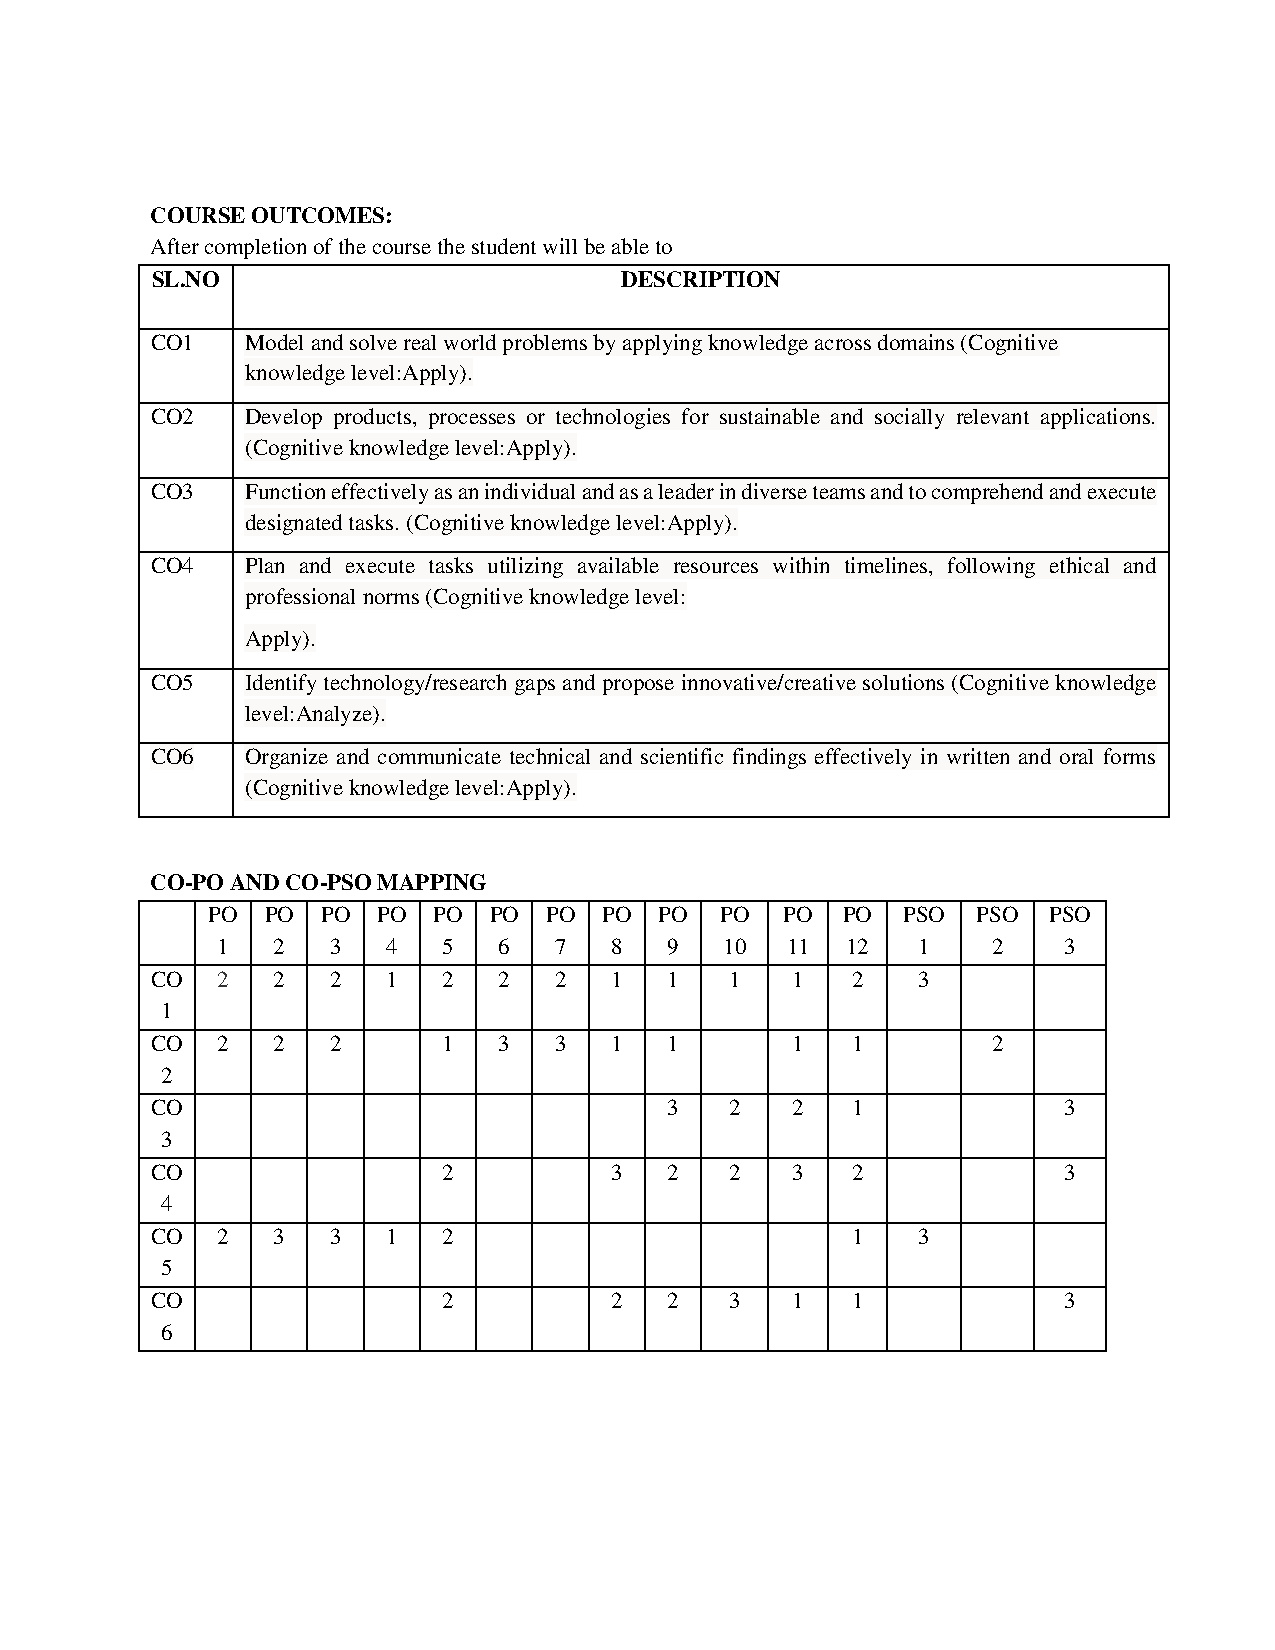
\includepdf[pages=-]{CO & jUSTIFICATIONS.pdf}
	
	\clearpage

\clearpage

% \addcontentsline{toc}{chapter}{Appendix D: CO-PO-PSO Mapping}
% \chapter*{}
% \paragraph\
% \vspace{75mm}
% \begin{center}
%     \textbf{\huge{Appendix D: }}
%     \textbf{\huge{CO-PO-PSO Mapping}}
% \end{center}
% \clearpage
% \clearpage





\vspace{1cm}

\begin{table}[htp]
\centering
\caption*{CO-PO AND CO-PSO MAPPING}
\scalebox{0.75}{
\begin{tabular}{|p{0.8cm}|p{0.8cm}|p{0.8cm}|p{0.8cm}|p{0.8cm}|p{0.8cm}|p{0.8cm}|p{0.8cm}|p{0.8cm}|p{0.8cm}|p{0.8cm}|p{0.8cm}|p{0.8cm}|p{0.8cm}|p{0.8cm}|p{0.8cm}|}
\hline
\textbf{} & \textbf{PO
1} & \textbf{PO
2} & \textbf{PO
3} & \textbf{PO
4} & \textbf{PO
5} & \textbf{PO
6} & \textbf{PO
7} & \textbf{PO
8} & \textbf{PO
9} & \textbf{PO
10} & \textbf{PO
11} & \textbf{PO
12} & \textbf{PSO
1} & \textbf{PSO
2} & \textbf{PSO
3} \\
\hline
\textbf{CO
1} & 2 & 2 & 2 & 1 & 2 & 2 & 2 & 1 & 1 & 1 & 1 & 2 & 3 & & \\ \hline
\textbf{CO
2} & 2 & 2 & 2 & & 1 & 3 & 3 & 1 & 1 & & 1 & 1 & & 2 & \\ \hline
\textbf{CO
3} & & & & & & & & & 3 & 2 & 2 & 1 & & & 3 \\ \hline
\textbf{CO
4} & & & & & 2 & & & 3 & 2 & 2 & 3 & 2 & & & 3 \\ \hline
\textbf{CO
5} & 2 & 3 & 3 & 1 & 2 & & & & & & & 1 & 3 & & \\ \hline
\textbf{CO
6} & & & & & 2 & & & 2 & 2 & 3 & 1 & 1 & & & 3 \\
\hline
\end{tabular}}
\end{table}



\clearpage
\thispagestyle{plain}
\begin{center}
    \large{\textbf{JUSTIFICATIONS FOR CO-PO MAPPING}}
\end{center}

\begin{longtable}{|p{4.5cm}|p{1.5cm}|p{8.5cm}|}
\hline
\textbf{Mapping ID} & \textbf{Level} & \textbf{Justification} \\
\hline
\endfirsthead
% \multicolumn{3}{c}{\tablename\ \thetable\ -- Continued} \\
\hline
\textbf{Mapping ID} & \textbf{Level} & \textbf{Justification} \\
\hline
\endhead
\hline
\endfoot
\hline
\endlastfoot

101003/ CS722U.1-PO1 & M & Knowledge in the area of technology for project development using various tools results in better modeling. \\ \hline
101003/ CS722U.1-PO2 & M & Knowledge acquired in the selected area of project development can be used to identify, formulate, review research literature, and analyze complex engineering problems reaching substantiated conclusions. \\ \hline
101003/ CS722U.1-PO3 & M & Can use the acquired knowledge in designing solutions to complex problems. \\ \hline
101003/ CS722U.1-PO4 & M & Can use the acquired knowledge in designing solutions to complex problems. \\ \hline
101003/ CS722U.1-PO5 & H & Students are able to interpret, improve and redefine technical aspects for design of experiments, analysis and interpretation of data, and synthesis of the information to provide valid conclusions. \\ \hline
101003/ CS722U.1-PO6 & M & Students are able to interpret, improve and redefine technical aspects by applying contextual knowledge to assess societal, health and consequential responsibilities relevant to professional engineering practices. \\ \hline
101003/ CS722U.1-PO7 & M & Project development based on societal and environmental context solution identification is the need for sustainable development. \\ \hline
101003/ CS722U.1-PO8 & L & Project development should be based on professional ethics and responsibilities. \\ \hline
101003/ CS722U.1-PO9 & L & Project development using a systematic approach based on well defined principles will result in teamwork. \\ \hline
101003/ CS722U.1-PO10 & M & Project brings technological changes in society. \\ \hline
101003/ CS722U.1-PO11 & H & Acquiring knowledge for project development gathers skills in design, analysis, development and implementation of algorithms. \\ \hline
101003/ CS722U.1-PO12 & H & Knowledge for project development contributes engineering skills in computing \& information gatherings. \\ \hline

101003/ CS722U.2-PO1 & H & Knowledge acquired for project development will also include systematic planning, developing, testing and implementation in computer science solutions in various domains. \\ \hline
101003/ CS722U.2-PO2 & H & Project design and development using a systematic approach brings knowledge in mathematics and engineering fundamentals. \\ \hline
101003/ CS722U.2-PO3 & H & Identifying, formulating and analyzing the project results in a systematic approach. \\ \hline
101003/ CS722U.2-PO5 & H & Systematic approach is the tip for solving complex problems in various domains. \\ \hline
101003/ CS722U.2-PO6 & H & Systematic approach in the technical and design aspects provide valid conclusions. \\ \hline
101003/ CS722U.2-PO7 & H & Systematic approach in the technical and design aspects demonstrate the knowledge of sustainable development. \\ \hline
101003/ CS722U.2-PO8 & M & Identification and justification of technical aspects of project development demonstrates the need for sustainable development. \\ \hline
101003/ CS722U.2-PO9 & H & Apply professional ethics and responsibilities in engineering practice of development. \\ \hline
101003/ CS722U.2-PO11 & H & Systematic approach also includes effective reporting and documentation which gives clear instructions. \\ \hline
101003/ CS722U.2-PO12 & M & Project development using a systematic approach based on well defined principles will result in better teamwork. \\ \hline

101003/ CS722U.3-PO9 & H & Project development as a team brings the ability to engage in independent and lifelong learning. \\ \hline
101003/ CS722U.3-PO10 & H & Identification, formulation and justification in technical aspects will be based on acquiring skills in design and development of algorithms. \\ \hline
101003/ CS722U.3-PO11 & H & Identification, formulation and justification in technical aspects provides the betterment of life in various domains. \\ \hline
101003/ CS722U.3-PO12 & H & Students are able to interpret, improve and redefine technical aspects with mathematics, science and engineering fundamentals for the solutions of complex problems. \\ \hline

101003/ CS722U.4-PO5 & H & Students are able to interpret, improve and redefine technical aspects with identification formulation and analysis of complex problems. \\ \hline
101003/ CS722U.4-PO8 & H & Students are able to interpret, improve and redefine technical aspects to meet the specified needs with appropriate consideration for the public health and safety, and the cultural, societal, and environmental considerations. \\ \hline
101003/ CS722U.4-PO9 & H & Students are able to interpret, improve and redefine technical aspects for design of experiments, analysis and interpretation of data, and synthesis of the information to provide valid conclusions. \\ \hline
101003/ CS722U.4-PO10 & H & Create, select, and apply appropriate techniques, resources, and modern engineering and IT tools for better products. \\ \hline
101003/ CS722U.4-PO11 & M & Students are able to interpret, improve and redefine technical aspects by applying contextual knowledge to assess societal, health and consequential responsibilities relevant to professional engineering practices. \\ \hline
101003/ CS722U.4-PO12 & H & Students are able to interpret, improve and redefine technical aspects for demonstrating the knowledge of, and need for sustainable development. \\ \hline

101003/ CS722U.5-PO1 & H & Students are able to interpret, improve and redefine technical aspects, apply ethical principles and commit to professional ethics and responsibilities and norms of engineering practice. \\ \hline
101003/ CS722U.5-PO2 & M & Students are able to interpret, improve and redefine technical aspects, communicate effectively on complex engineering activities with the engineering community and with society at large, such as, being able to comprehend and write effective reports and design documentation, make effective presentations, and give and receive clear instructions. \\ \hline
101003/ CS722U.5-PO3 & H & Students are able to interpret, improve and redefine technical aspects to demonstrate knowledge and understanding of the engineering and management principles in multidisciplinary environments. \\ \hline
101003/ CS722U.5-PO4 & H & Students can interpret, improve and redefine technical aspects, recognize the need for, and have the preparation and ability to engage in independent and life-long learning in the broadest context of technological change. \\ \hline
101003/ CS722U.5-PO5 & M & Students are able to interpret, improve and redefine technical aspects in acquiring skills to design, analyze and develop algorithms and implement those using high-level programming languages. \\ \hline
101003/ CS722U.5-PO12 & M & Students are able to interpret, improve and redefine technical aspects and contribute their engineering skills in computing and information engineering domains like network design and administration, database design and knowledge engineering. \\ \hline

101003/ CS722U.6-PO5 & M & Students are able to interpret, improve and redefine technical aspects and develop strong skills in systematic planning, developing, testing, implementing and providing IT solutions for different domains which help in the betterment of life. \\ \hline
101003/ CS722U.6-PO8 & H & Students will be able to associate with a team as an effective team player for the development of technical projects by applying the knowledge of mathematics, science, engineering fundamentals, and an engineering specialization to the solution of complex engineering problems. \\ \hline
101003/ CS722U.6-PO9 & H & Students will be able to associate with a team as an effective team player for Identify, formulate, review research literature, and analyze complex engineering problems. \\ \hline
101003/ CS722U.6-PO10 & M & Students will be able to associate with a team as an effective team player for designing solutions to complex engineering problems and design system components. \\ \hline
101003/ CS722U.6-PO11 & M & Students will be able to associate with a team as an effective team player using research-based knowledge and research methods including design of experiments, analysis and interpretation of data. \\ \hline
101003/ CS722U.6-PO12 & H & Students will be able to associate with a team as an effective team player, applying ethical principles and committing to professional ethics and responsibilities and norms of engineering practice. \\ \hline
101003/ CS722U.1-PSO1 & H & Students can develop Computer Science Specific Skills by modeling and solving problems. \\ \hline
101003/ CS722U.2-PSO2 & M & Developing products, processes or technologies for sustainable and socially relevant applications can promote Programming and Software Development Skills. \\ \hline
101003/ CS722U.3-PSO3 & H & Working in a team can result in the effective development of Professional Skills. \\ \hline
101003/ CS722U.4-PSO3 & H & Planning and scheduling can result in the effective development of Professional Skills. \\ \hline
101003/ CS722U.5-PSO1 & H & Students can develop Computer Science Specific Skills by creating innovative solutions to problems. \\ \hline
101003/ CS722U.6-PSO3 & H & Organizing and communicating technical and scientific findings can help in the effective development of Professional Skills. \\ \hline
\end{longtable}
	
\end{document}